% REMEMBER: You must not plagiarise anything in your report. Be extremely careful.

\documentclass{l4proj}

    
%
% put any additional packages here
%

\begin{document}

%==============================================================================
%% METADATA
\title{Machine Learning models with Natural Language Processing as a usable online tool for fake news detection}
\author{Kārlis Siders}
\date{March ?? 2023}

\maketitle

%==============================================================================
%% ABSTRACT
\begin{abstract}
    % Every abstract follows a similar pattern. Motivate; set aims; describe work; explain results.
    % \vskip 0.5em
    % ``XYZ is bad. This project investigated ABC to determine if it was better. 
    % ABC used XXX and YYY to implement ZZZ. This is particularly interesting as XXX and YYY have
    % never been used together. It was found that  
    % ABC was 20\% better than XYZ, though it caused rabies in half of subjects.''
    With the increasing spread of fake news on all online social media platforms and the difficulty of detecting fake news by the average social media user, there is a need for automatic detection methods to be used to keep the integrity of news shared online. This necessity is currently exacerbated on Twitter, a source of news for many, with its changing leadership roles and, consequently, policies. Since there is much literature about different solutions to the problem, this paper aims to describe the general problem at large, the various concepts used in other literature, and describe the requirements-gathering, design, implementation, and evaluation stages of such a project. The project investigated how two Machine Learning algorithms, Logistic Regression and BERT, can be made and trained using Natural Language Processing techniques to detect fake news in Tweets, with the unique nature of building and sharing a usable tool for users to access. While the Logistic Regression algorithm achieves only 82.8\% accuracy (with an F1 score of 82.6\%), BERT achieves an accuracy of 99.2\% (and an F1 score of 99.4\%), which, while being impressive for the given dataset, is not generalisable much to modern Tweets.
    
\end{abstract}

%==============================================================================

% EDUCATION REUSE CONSENT FORM

\def\consentname {Kārlis Siders} % your full name
\def\consentdate {21 January 2023} % the date you agree

\educationalconsent



%==============================================================================
\tableofcontents

%==============================================================================
%% Notes on formatting
%==============================================================================
% The first page, abstract and table of contents are numbered using Roman numerals and are not
% included in the page count. 
%
% From now on pages are numbered
% using Arabic numerals. Therefore, immediately after the first call to \chapter we need the call
% \pagenumbering{arabic} and this should be called once only in the document. 
%
% Do not alter the bibliography style.
%
% The first Chapter should then be on page 1. You are allowed 40 pages for a 40 credit project and 30 pages for a 
% 20 credit report. This includes everything numbered in Arabic numerals (excluding front matter) up
% to but excluding the appendices and bibliography.
%
% You must not alter text size (it is currently 10pt) or alter margins or spacing.
%
%
%==================================================================================================================================
%
% IMPORTANT
% The chapter headings here are **suggestions**. You don't have to follow this model if
% it doesn't fit your project. Every project should have an introduction and conclusion,
% however. 
%
%==================================================================================================================================
\chapter{Introduction}

% reset page numbering. Don't remove this!
\pagenumbering{arabic} 

\section{Motivation}

Fake news is a concept that every Internet user knows all too well because of its rapid spread over every social media platform and forum. Journalists and researchers have been actively searching and developing ways to minimise the spread, and many organisations have been created just for the purpose of identifying and spreading awareness about popular fake news online. For example, the popular PolitiFact platform uses real people (the reporter who researchers and writes about a specific topic and two editors who check both the writing and the assigned category of truth in their own scale called the Truth-O-Meter\footnote{This robust method of research is also the reason why I decided to use the dataset containing their data in my model.}) to identify fake news \citep{PolitiFact}. However, with the growing spread of fake news, the sheer amount cannot all be analysed by a dedicated team of researchers, which is why a machine learning model which can analyse any number of texts with measurable accuracy is one of the optimal solutions to detecting fake news.

There are many articles online to help people distinguish between fake and real news \citep{FakeRealHelp}, which essentially define the relevant terms, describe critical thinking and do nothing else. What I wanted to do was give a real tool for people to use and determine whether a post is likely to be fake news or not.

With Twitter being taken over by Elon Musk, who seemingly does not care about the spread of disinformation as Twitter has "stopped enforcing its policy on misleading information about coronavirus" \citep{TwitterCovid}, the detection of fake news has become ever more important, especially on Twitter. 


\section{Goals}

\subsubsection{Machine Learning Model with Natural Language Processing}

Build an ML model that uses NLP to analyse the text and other features of Tweets in order to make a decision about whether it is fake news or not. The model should use modern technology with some of the latest developments in both machine learning and natural language processing in order to achieve higher accuracy and be usable.

\subsubsection{Better Than Human Performance}
Because the average Internet user can correctly distinguish between fake and real news with only 54\% accuracy \citep{FakeNewsTrends}, the model's accuracy and F1 score\footnote{Explained in section \ref{subsubsec:F1}.} should be better than 54\% in order for the tool to be at all useful for users. 

\subsubsection{Two Comparable Models}
\label{subsec:goal_two_models}
Have two models, one that uses Twitter API to get multiple features from a Tweet and one that uses only text, which in turn can be generalised for any text. The former, more complex, model would depend on Twitter API, which would make it dependent on any ongoing changes at Twitter, and with Twitter's micro-services being at risk \citep{Twitter2FA}, the model could turn out to be unusable in the future. Therefore, the smaller, simpler, model would act as a more stable backup model.

\subsubsection{Online Tool}
Build and host a website that hosts the models built previously for Internet users to access and be able to predict the veracity of text and/or Tweets. The website should be easily navigable and understandable for users without any knowledge of machine learning or natural language processing to use.

\section{Structure}

\textbf{Chapter \ref{chap:background}} gives the existing definitions of fake news, explains the core concepts behind the project, along with a review of existing solutions for similar research problems and their limitations.

\textbf{Chapter \ref{chap:anal}} discusses the problem space of the project and how it was discovered and analysed.

\textbf{Chapter \ref{chap:design}} outlines how the solution to the problem was designed with the core elements of the project highlighted, including dataset acquiescence, NLP pre-processing, building of the ML model, validation of the model, evaluation, and building of a tool that uses this model.

\textbf{Chapter \ref{chap:implem}} discusses the many parts of implementing the solution to the problem, including dataset analysis and cleaning using traditional and NLP techniques, ML model choosing and implementing, and Django website building.

\textbf{Chapter \ref{chap:eval}} explains how the model and website were evaluated using the appropriate evaluation methods, including the confusion matrix and different accuracy scores for the model.

Finally, \textbf{chapter \ref{chap:conclusion}} summarises the project's problem, solution, and its effectiveness with the limitations highlighted.


% Why should the reader care about what are you doing and what are you actually doing?


% \section{Guidance}

% \textbf{Motivate} first, then state the general problem clearly. 

% \section{Writing guidance}
% \subsection{Who is the reader?}

% This is the key question for any writing. Your reader:

% \begin{itemize}
%     \item
%     is a trained computer scientist: \emph{don't explain basics}.
%     \item
%     has limited time: \emph{keep on topic}.
%     \item
%     has no idea why anyone would want to do this: \emph{motivate clearly}
%     \item
%     might not know \emph{anything} about your project in particular:
%     \emph{explain your project}.
%     \item
%     but might know precise details and check them: \emph{be precise and
%     strive for accuracy.}
%     \item
%     doesn't know or care about you: \emph{personal discussions are
%     irrelevant}.
% \end{itemize}

% Remember, you will be marked by your supervisor and one or more members
% of staff. You might also have your project read by a prize-awarding
% committee or possibly a future employer. Bear that in mind.


% \subsubsection{Citation styles}

% \begin{itemize}
% \item If you are referring to a reference as a noun, then cite it as: ``\citet{Orw68} discusses the role of language in political thought.''
% \item If you are referring implicitly to references, use: ``There are many good books on writing \citep{Orw68, Wil09, Pin15}.''
% \end{itemize}

% There is a complete guide on good citation practice by Peter Coxhead available here: \url{http://www.cs.bham.ac.uk/~pxc/refs/index.html}. 
% If you are unsure about how to cite online sources, please see this guide: \url{https://student.unsw.edu.au/how-do-i-cite-electronic-sources}.


%==================================================================================================================================
\chapter{Background}
\label{chap:background}
% What did other people do, and how is it relevant to what you want to do?

\section{Fake News Definition}

Fake news is a concept with a large spectrum of definitions that remain contested by academics and are ever evolving to keep up with new ways in which false information is spread online. Defined earlier as "fabricated information that mimics news media
content in form but not in organizational process or intent" by \cite{FakeNewsScience} 
and later as "synonymous with the spread of false information on social media" by 
\cite{FakeNewsTrends}, it is a concept ripe for grey areas, with unclear boundaries around whether omissions and exaggerations of fact amount to fake news. However, the nature of it is clearer: its spread over the Internet is rapid, and researchers have been developing methods to counteract it for decades. This chapter describes the technical background necessary for the project, and existing solutions to combat fake news.

\section{Technical Explanations}

\subsection{Machine Learning}

Machine learning (ML) has developed with huge leaps in the last few decades, with new applications of machine learning models being found every day. Because of improvements in CPU and GPU performance, new ML model efficiency, and digitalisation of environmental data, machine learning can be and has been used for an increasing amount of projects to improve many aspects of life.

ML can be split into three main parts: supervised learning, where there is labelled data that a model learns from and tries to understand the underlying relationships between the input and the expected output; unsupervised learning, where the goal is mostly to find similarities between items and group them; and reinforcement learning, where there are general metrics that the model tries to improve based on trial and error while interacting with some environment, like autonomous driving \citep{MLTypes}. Because the project is about classifying social media posts, supervised learning is what this paper will focus on.


\subsection{Natural Language Processing}
\label{subsec:NLP}

In order for any ML model to learn to understand human language, the input text needs to first be processed with Natural Language Processing (NLP) techniques. NLP in machine learning has largely been developed with the goal of perfecting machine translation in mind; however, there are many other applications in the last decade, including image captioning, web search, and speech understanding \citep{NLPIntro}.

These techniques are all applied sequentially in what is usually called an NLP pipeline. The pipeline consists of tokenisation, stop word removal, and vectorisation, among other more optional stages.

\subsubsection{Tokenisation}

The very first step of the NLP pipeline is tokenisation as it is necessary to first transform the unstructured data that is text into some sort of structured data, in this case tokens. Tokens are collected by splitting larger sentences into standardised parts, like words, punctuation, and sentence separators.

\subsubsection{Stop Word Removal}

In order to remove clutter that does not add much value to the meaning of a sentence, certain words which do not mean much, like "the", "is", "are", etc, are removed from the text. These are called stop words. Most often, these words are kept in a long list that is compared against the text because there is no detectable characteristic attributable to them all except for their minimal meaning in a sentence.

\subsubsection{Vectorisation}

Because models need input in the format of numbers, the previously acquired tokens need to be translated into a numerical representation, i.e., vectorised. There are many vectorising approaches available, but the one used in this project is the TF-IDF vectoriser. This vectoriser balances two important concepts: term frequency (TF) and document frequency (DF). Term frequency is the idea that the more frequently a certain word appears in a sentence, the more important it is\footnote{This is why stop word removal is essential for most vectorisers; otherwise, "the" would be the most important word of all in English.}. Document frequency balances out topic-specific words by counting how many documents (in this case, sentences) contain the token, which might be important if all of the sentences have similar topics, e.g., if the dataset is of political Tweets, the term "party" might not be as important as "corrupt", even though the former appears more often than the latter. Because of this inverse relationship, inverse document frequency (IDF) is used. If $df_t$ is the document frequency of token $t$ and $N$ is the total number of documents, then inverse document frequency of token $t$ is

\[idf_t = \log(\frac{N}{df_t}).\]

TF-IDF is then added as a weight to the token thus:

\[w_{t,d} = (1 + \log{(tf_{t,d})}) \cdot \log{(\frac{N}{idf_t})},\]

where $tf_{t,d}$ is the term frequency of token $t$ in document $d$.


\subsection{Machine Learning Models}

There is an abundance of ML models used in both research and business in all types of machine learning, but the main types of models in supervised learning are for classification (labelling items as belong to one or more categories), regression (finding dependency between independent and dependent variables), and forecasting (predicting future behaviour based on past data). Since the aim of the project is to label social media posts as fake or real news, this section will focus on the two classification models used throughout the project.

\subsubsection{Logistic Regression}

Logistic Regression is one of the most widely used ML classifiers since it can easily be used for binary classification, which is also applicable for this project. The model works well because it fits the input data to a sigmoid curve, as seen in Figure \ref{fig:LRSigmoid}, which can be used to classify the given data into two classes based on one or more features according to how much the given values for the features lean one way or the other \citep{LogRegression}.

\begin{figure}
    \centering
    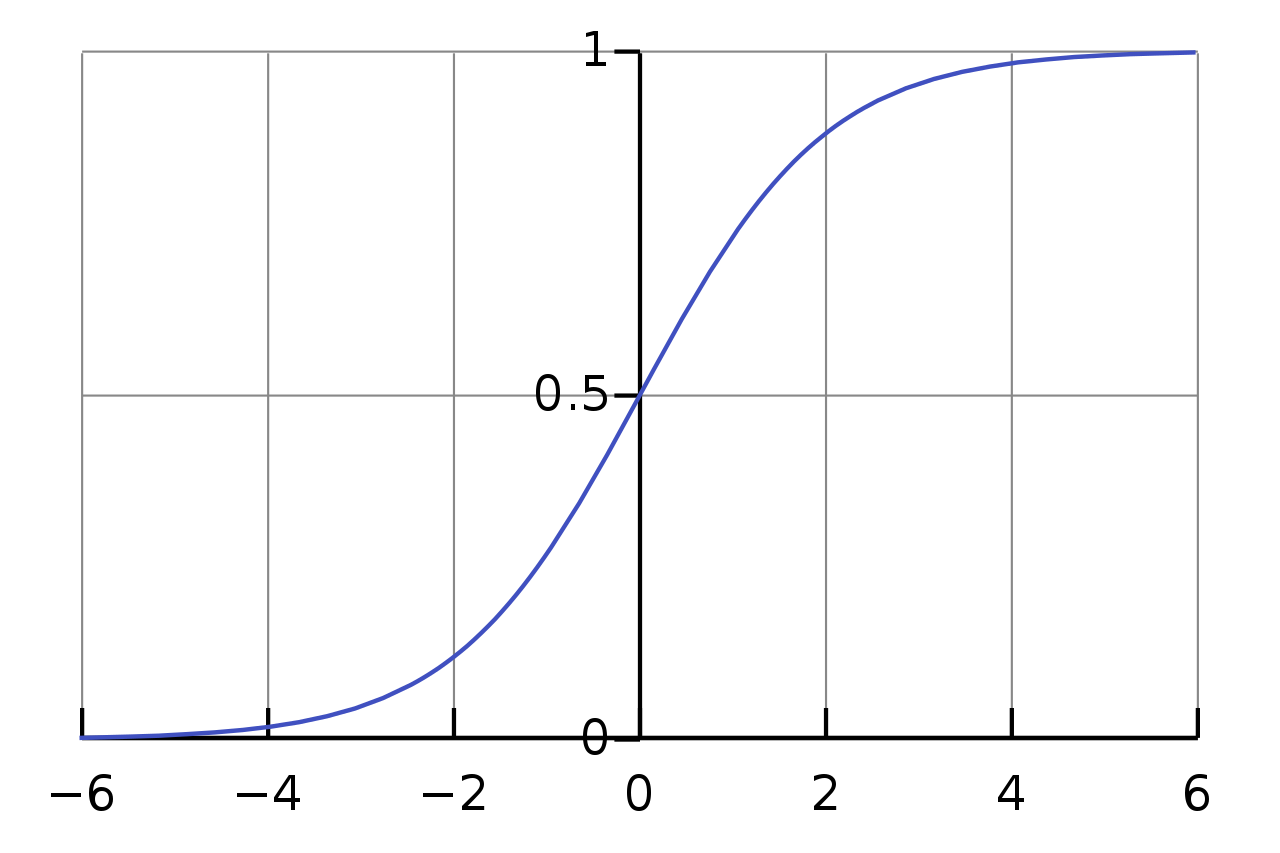
\includegraphics[width=0.5\linewidth]{images/Background/sigmoid.png}    

    \caption{The sigmoid activation function used by Logistic Regression as made by \citet{LRSigmoid}.}
    \label{fig:LRSigmoid} 
\end{figure}

\subsubsection{Transformer}

Introduced in 2017 by \citeauthor{NLPTransformer}, the transformer is the state-of-the-art model used in every modern NLP project. Although it is just another machine learning architecture, typically with encoders and decoders both using the Feed Forward Neural Network (FFNN), and word embeddings, what distinguishes it from previous models used in NLP, like Long Short-Term Memory (LSTM) networks and other Recurrent Neural Networks (RNNs), is the addition of self-attention \citep{TransformerExplained}. Attention, visible in Figure \ref{fig:transformer}, is a method of dealing with long-range dependencies of words in sentences by keeping track of the distances between dependent words and adding them to the weight of the tokens. The previously mentioned FFNN is a massive neural network included in both the encoder and decoder stacks, and it is unique in the fact that it does not have any backpropagation for changing the weights of the network, the information goes only one way. Word embeddings are a way to add meaning to words by representing the different features of them (acquired by analysing the context that they usually appear in) with numbers. A list of these word embeddings is used when training the model, which is usually a so-called vocabulary of tens of thousands of words. The transformer architecture has gained its popularity thanks to the extremely effective combination of already existing components (the FFNN, tokenisation, word embeddings, encoder and decoder stacks, linear classifiers for probability calculation at the end of the architecture's output) and new technologies (self-attention).

\begin{figure}
    \centering
    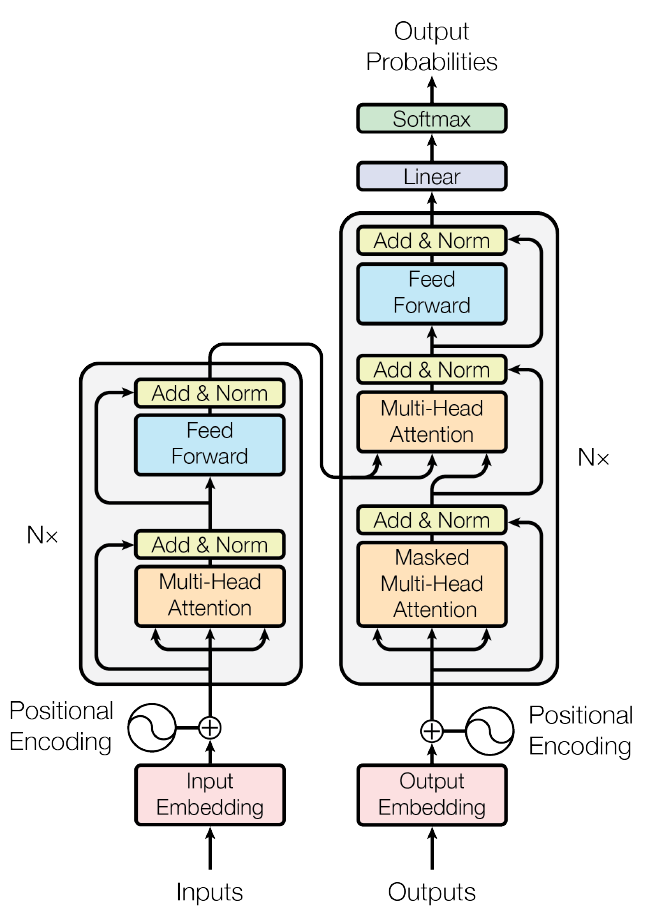
\includegraphics[width=0.5\linewidth]{images/Background/transformer.png}    

    \caption{The architecture of the first-ever transformer proposed by \cite{NLPTransformer} from Google Brain and co.}
    \label{fig:transformer} 
\end{figure}


\subsection{BERT}

Bi-directional Encoder Representations for Transformers (BERT) is an ML model with a transformer architecture that was published in 2018 by the team at Google (\citeauthor{BERT}). What distinguishes BERT from a typical transformer is its bi-directionality of context (looking both right and left of a word in a sentence to determine its context), achieved by using transformer encoders for word embeddings and masking (hiding some words from a sentence and having the model guess which words have been hidden) without any decoder stack \citep{BERTExplained}. Another "game" that the model has learnt sentence structure by is from replacing some words with other words and seeing if the model can guess, firstly, which words are out of place, and secondly, what words should be there instead.

The power of BERT is evident from the way it is used in machine learning projects. When it is imported, it is already pre-trained from 800 million words in a collection of text documents (corpus) called BooksCorpus \citep{BERT}, collected from 11 films and the books that they are based on \citep{BooksCorpus}. The task of each project is not to use BERT from scratch, but to do further training with a dataset and a specific task (like classification), the process of which is called fine-tuning.

The activation function that BERT uses is GELU (Gaussian Error Linear Unit) because the "small non-linearity [in] the negative range helps maintain the long relation tracking [...] in BERT" \citep{BERTGELU}, seen in Figure \ref{fig:BERTGELU}.

\begin{figure}
    \centering
    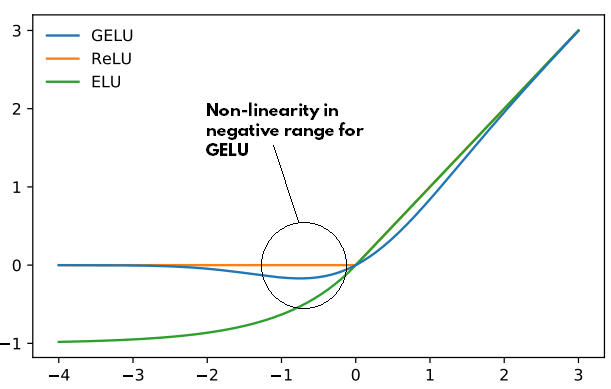
\includegraphics[width=0.8\linewidth]{images/Background/BERT GELU.png}    

    \caption{The different Linear Unit functions compared, with the negative dip in GELU emphasised by \citet{BERTGELUFigure}.}
    \label{fig:BERTGELU} 
\end{figure}


\subsection{Machine Learning Model Evaluation Metrics}

After an ML model has been built and fine-tuned, its performance needs to be evaluated by having it predict the labels of a test dataset that it has not seen before and comparing the predictions with the true dataset. There are different metrics that can be used, some with more drawbacks than others, but the following is a summary of the most prevalent ones for binary classification.

\subsubsection{Accuracy}

The simplest measure of performance, accuracy, is defined as the count of correct predictions divided by all predictions. However, this metric suffers from the Class Imbalance problem, which is the case when one class/category is more prevalent than the other, e.g., real news being more frequent than fake news. In such a case the model might learn to predict only the majority class, and this would result in a high accuracy. If $T$ and $F$ stand for 'True' and 'False', e.g., correctly and incorrectly predicted, and $P$ and $N$ stand for 'Positive' and 'Negative', e.g., real and fake news, then accuracy can be defined as

\[A=\frac{TP+TN}{TP+TN+FP+FN}.\]

\subsubsection{Precision}

The definition of precision can be seen as the "exactness" of a model, i.e., of all of the predictions about one class, e.g., real news, how many were correct. This metric encourages the model to make fewer unsafe predictions since just one correct prediction would result in 100\% accuracy as the formula for precision is

\[P_r=\frac{TP}{TP+FP}.\]

\subsubsection{Recall}

The antithesis of precision, recall, measures the "completeness" of the model, i.e., how many predictions of the total amount of a class, e.g., real news, the model predicted correctly. Because this metric does not measure incorrect predictions, it encourages the model to make more unsafe predictions to be more "complete" since the formula for it is 

\[R=\frac{TP}{TP+FN}.\]

\subsubsection{F1}
\label{subsubsec:F1}

The F1 score of a model is a metric that combines both precision and recall to find a balance for both. Therefore, the formula for that is the harmonic mean of both, i.e., 

\[F_1=\frac{2\cdot P_r\cdot R}{P_r + R}=\frac{2TP}{2TP + FP + FN}.\]

\subsubsection{Confusion Matrix}
\label{subsec:conf_matrix}

The confusion matrix is a simple 2x2 table showing the counts for all of TP, TN, FP, and FN, usually with a coloured gradient to help visualise the difference in the amounts. This table is useful for identifying whether or how much any correct or incorrect predictions are unbalanced, and the metric for the models of the project can be found in section \ref{sec:ConfMatrix}.

\section{Existing Solutions}

Because of the decades of research in the aforementioned fields, this section summarises the relevant research in machine learning and natural language processing in classification tasks, and the limitations that this project tries to rectify.

\subsection{ML in Classification}

ML has been used to classify a diverse range of items in a lot of fields, including health care, cyber security, and abundantly in NLP \citep{MLApps}. In cyber security, ML classification has helped distinguish between malware and harmless software. In health care, ML classification has been used to label tumours as either benign or malignant. Both classifications used multiple features to analyse the behaviour and nature of the items, but neither used NLP since the features did not include natural language. However, as described by \citeauthor{MLApps}, NLP is an important and highly frequent co-requisite for ML classification tasks.


\subsection{NLP in Classification}

The one example of NLP in \cite{MLApps} is, coincidentally, also of Tweet classification. The researchers labelled Tweets as originating either from Hillary Clinton or Donald Trump, two prominent actors in the American political sphere, using NLP techniques to pre-process the lexical data, including a hash vectoriser, which, hashing the term frequency only, does not account for (inverse) document frequency \citep{scikit-learn}. The model used in this example was XGBoost, a version of the gradient boosted trees algorithm used in many other ML projects.

There have also been attempts to generalise NLP-based detection for a topic-agnostic model \citep{Topic-AgnosticIdentification}, which used certain pre-processing techniques that have been adapted in this project, like NLTK pre-processing.

Apart from the models themselves and as can be seen from Table 2 in the NLP review done by \cite{FakeNewsTrends}, there have been a multitude of datasets made by researchers, with different types of content (social media posts, short statements, and whole articles), quantity (from 330 posts to 60 million posts), labelling scale of veracity (from binary to six levels), and annotators (crowd-sourcing, journalistic teams, or news agencies). 


\subsection{Limitations}
Almost none of the solutions I have found offer a practical tool for non-technical
people (either researchers or programmers who can replicate the code in the research papers) to actually use\footnote{Although there is one model I found, the model made by \cite{ThaiModel} is in Thai.}. Even though research papers do not usually include the possible implementations of their models, this paper focuses not only on the creation of the NLP ML model, but also on the practical aspects of implementing it in a Django-hosted web application. 

The other limitation of the research is that only a small portion discuss at length the dataset that they use for training the model, which is among the most important aspects of the model because it can highlight biases and skewed perspectives apparent in the dataset. This I have also tried to rectify in the paper.

%==================================================================================================================================
\chapter{Requirements}
\label{chap:anal}
% What is the problem that you want to solve, and how did you arrive at it?
% \section{Guidance}
% Make it clear how you derived the constrained form of your problem via a clear and logical process. 

The problem to be solved, as stated in the introduction, arises from the increase of fake news spread online, and was proposed by Dr Chris McCaig, a lecturer at the University of Glasgow. The requirements of the solution to the problem are detailed below using the MoSCoW method, a prioritisation technique frequently used in software development and other fields. The prioritisation (most to least important) is thus: \textit{Must Have}, \textit{Should Have}, \textit{Could Have}, and \textit{Will not Have}. The requirements are also split into functional and non-functional requirements, explained below.

\section{Functional Requirements}

Functional requirements are the active aspects of a software system that users interact with and can see the use of. Discussed below are the functional requirements gathered with the project's supervisor.

\textbf{Must Have:}
\begin{itemize}
    \item The very first requirement of training a classifying ML model is the acquisition of a dataset with labelled data. This allows the model to learn the characteristics of fake Tweets and real ones and build a network to determine the difference between the two classes.  
    \item After a dataset is acquired, an ML model needs to be built to get the dataset as an input and learn from it.
    \item The model must be built into a usable tool in order to give it a Tweet or a piece of text from a Tweet and receive back a prediction determining whether it is fake news or not.
\end{itemize}

\textbf{Should Have:}
\begin{itemize}
    \item The tool that uses the model should be built as a web application for easier use by non-technical users.
    \item The web application should be hosted on a domain that is accessible by the average user, not just by university staff or students.
\end{itemize}

\textbf{Could Have:}
\begin{itemize}
    \item There could be an option for a user to choose either of the two models for fake news detection, based on how they want to use it, i.e., either text-only or by using different features that can be acquired from Twitter API. This could be a useful feature for extensibility, but is not required by any means.
    \item It would be beneficial for the user to see what exactly was analysed from their input to the model which predicts the veracity of the input. For example, if the user includes a link to a Tweet, the website could show the text of the Tweet, the author's username, description, and verification status. This would increase the explainability of the model's prediction.
\end{itemize}

\textbf{Will not Have:}
\begin{itemize}
    \item Once a prediction has been given to the user's submitted input text/Tweet, the tool could have input for feedback about how well the model did, i.e., whether the prediction was accurate or not, and fit the model according to the new input. However, this could be complicated to implement and could easily be subject to abuse by users who purposely flag fake news as real news or vice versa. 
    \item It was discussed that the tool could be in a different form than a website - a browser extension. However, it was also decided that browser extensions, while being more bespoke and easier to adapt to a specific website, are too narrow in their features, which might be crucial if or when Twitter API and UI change, while also being less understandable and accessible to non-technical users, most of which know what websites are but only some of which are aware of browser extensions.
\end{itemize}

\section{Non-Functional Requirements}
\label{sec:non-func_reqs}

Non-functional requirements are the attributes of the software system that are required, i.e., characteristics that improve the quality, performance, and effectiveness of the project, but do not do so in a very visible way to the general user. Discussed below are the non-functional requirements gathered with the project's supervisor.

\textbf{Must Have:}
\begin{itemize}
    \item As stated above by \citet{FakeNewsTrends}, the average Internet user has about 54\% accuracy when distinguishing fake news from real news. Therefore, the model must achieve at least this accuracy to be useful for Internet users; otherwise, there is no usable tool developed for the project.
    \item The speed at which the class for one item is predicted must be reasonable for a user not to give up on using the tool while it is in the process of predicting. 
\end{itemize}

\textbf{Should Have:}
\begin{itemize}
    \item While it is acceptable to experiment with datasets consisting of narrower topics, like Covid-19 or climate change, it would be preferable for the final dataset to be broader in scope for better generalisability, for example, if the dataset was about any political news.
    \item Very often the dataset that is used for training the model is imbalanced, i.e., one of the classes is more frequent than the other. This issue should be fixed either by replicating more instances of the minority class (by generating new ones or repeating existing ones) or by removing enough instances of the majority class to match the minority class. The latter should only be done when there are enough instances of the minority class to make the input to the model large enough for significant training.
    \item The model should use one of the most modern and efficient algorithms and architectures for both the Natural Language Processing and Machine Learning parts, e.g., BERT.
\end{itemize}

\textbf{Could Have:}
\begin{itemize}
    \item The more complicated Twitter model could use multiple features for fake news prediction, including description, username, and verified status of the author of the Tweet. This would be useful for more fine-grained prediction with possibilities for additional text, e.g., the description; however, it is only an improvement on the base model that would work well enough on just the text of the Tweet.
    \item The model could support tokenisation of emojis in the dataset since they can be a very important part of any text, clarifying or sometimes even changing semantics entirely (especially in the case of sarcasm, e.g., "I love how you never reply back..." if it is accompanied by an unamused emoji) \citep{EmojiSemantics}. However, most often emojis only add to the sentiment of the text, exclusively on which BERT has already been pre-trained.
    \item Regarding evaluation, the resulting confusion matrix of predicting fake news from the test dataset could be balanced in terms of incorrect predictions for each class. However, most often the confusion matrix is imbalanced, and there is not much that can be done to fix that.
\end{itemize}

\textbf{Will not Have:}
\begin{itemize}
    \item The model's performance could have 100\% accuracy for the given dataset. However, this is generally impossible and considered useless since it would always be over-fitted to the dataset and not be generalisable to completely new inputs.
\end{itemize}

%==================================================================================================================================
\chapter{Design}
\label{chap:design}
% How is this problem to be approached, without reference to specific implementation details? 
% \section{Guidance}
% Design should cover the abstract design in such a way that someone else might be able to do what you did, but with a different language or library or tool.

With the requirements in place, next it was time to design the project in such a way that they would be achieved with the MoSCoW prioritisation in mind. This chapter gives an overview of the aspects that such a project should include and explains the aspects in more detail.

\section{Overview}
\label{sec:design_overview}

The core elements of the project are outlined in Figure \ref{fig:design}. As can be seen in the diagram, the first part of the project will acquiring an appropriate dataset containing both fake and real news from items in a domain. After the initial acquisition, the dataset will need to be processed, both from a cleaning and transformation perspective in order to get text containing all features to be analysed and further processed for model input. These first steps regarding the dataset are explained in further detail in Section \ref{sec:design_dataset}. As soon as the text is acquired, it will be needing to be processed with Natural Language Processing techniques, the specifics of which are demonstrated in Section \ref{sec:design_NLP}, after which the input can be used for model training, detailed in Section \ref{sec:design_ML}. Finally, the models will be hosted on a web application, the building of which is outlined in Section \ref{sec:design_web}.

\begin{figure}
    \centering
    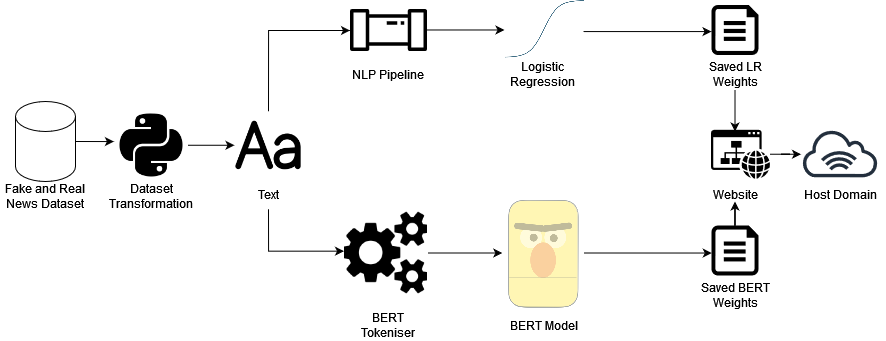
\includegraphics[width=1\linewidth]{images/diss-design-final.drawio.png}    

    \caption{The flow diagram of the project with the core elements\protect\footnotemark.}
    \label{fig:design} 
\end{figure}

\footnotetext{The BERT icon is taken from \citet{BERTExplained}.}

\section{Dataset Acquisition and Transformation}
\label{sec:design_dataset}

A dataset will be acquired, which is preferably domain-specific, like one containing only posts from Facebook or Tweets from Twitter, in order for it to perform better for a specific purpose since general all-purpose tools are very difficult to make. Next is one of the most critical parts of any Data Analysis project, as described by \citet{BigData}: investigation, exploration, transformation, and cleaning of the dataset.

With any division into classes, the balance of the dataset needs to be investigated and corrected, if necessary. If there is a significant imbalance in the counts of instances in the classes, there are two main approaches for the solution: either to generate more of the minority class to reach the number of majority class items (by replicating existing ones or generating new ones based on certain patterns in the existing ones) or to reduce the amount of the majority class by sampling random ones until the amount of the minority class is reached. The latter approach is faster and easier, but it does result in fewer items that the model can be trained on.

Oftentimes the dataset does not have the data prepared in the most appropriate format for how it is planned to be used in the project. For example, if the IDs of Tweets are in a list in one cell in the dataset and they need to be extracted for each row, this extraction is a form of transforming the dataset in order to get appropriate values.

Finally, dataset cleaning is very often necessary for any project since only rarely do researchers need all aspects of a dataset and often the unnecessary parts can be discarded. For example, if there are unnecessary index columns or insignificant IDs of the author of a post, those columns should be removed in order not to fill up memory unnecessarily when the dataset is loaded as a variable. The more in-depth cleaning of the text is detailed in the next section.

\section{Natural Language (Pre-)Processing}
\label{sec:design_NLP}

Once the dataset is cleaned, the text that will be the input to the Natural Language Processing model needs to be cleaned as well. This needs to be done according to the pipeline outlined in subsection \ref{subsec:NLP}, i.e., the text should be converted into being all-lowercase, tokenised, and stop words should be removed. Additionally, the text could go through the stemming process, which keeps only the roots of the words, e.g., "consult", "consultant", and "consulting" all turn into "consult", and also the lemmatisation process, which standardises the different possible forms of words, e.g., "is", "are", and "am" all turn into "be".

Afterwards, the prepared text can be vectorised with a TF-IDF vectoriser.

To note, this pre-processing stage is only necessary for the simpler model that is not implemented with BERT since the BERT model uses a BERT tokeniser that does everything mentioned above. However, more thought needs to be put into the parameters of the tokeniser, e.g., what the maximum length of all input items should be since the BERT model expects standardised input. This maximum length can be found by analysing all of the inputs that will be given to the model and either reducing or keeping the amount of the maximum length.

\subsection{BERT Tokeniser Parameters}
\label{subsec:BERTTokeniserParams}

\subsubsection{Attention Masks}

Because of the strict input standardisation for the BERT model, i.e., having all sentences be the same length, padding is used on the shorter sentences to lengthen them to be as long as the longest one. Attention masks are a simple but effective way for the model to know which tokens to pay attention to (the non-padded values) and which ones not to (the padded values) by representing both kinds of values as an array the length of the sentence, each value (1 or 0) being a label for the specific token in the order.

\subsubsection{Special Tokens}

When BERT was originally trained on 80 million terms, it was trained with special tokens that separated sentences in meaningful ways. The [CLS] token started each independent sentence to be classified (hence, CLS), and the [SEP] token separated two-sentence inputs when training BERT on next sentence prediction. Because of this format being used to pre-train the model, fine-tuning that does not involve more than 80 million terms is best done with the same format not to confuse the model. Therefore, the inclusion of these special tokens is almost always the best practice.

\section{Machine Learning Models}
\label{sec:design_ML}

After tokenising and vectorising the input (either manually or with the BERT tokeniser), it can be put into the models. The type of input will depend on which model will be used (TF-IDF vectorised representations for Logistic Regression, and BERT tokeniser-processed sentences for the BERT model). While training these models it is also important to keep a baseline model to compare the advanced models' performance against. There are many libraries in Python and other languages which provide this functionality.

For Logistic Regression, the input can just be fitted with simple commands in any language, then evaluated with accuracy, F1 score, and confusion matrix.

For BERT, many more decisions need to be made on the parameters for instantiating the model, like epoch size, batch size, and learning rate, detailed below.

\subsection{BERT Model Training Parameters}

\subsubsection{Epoch Amount}
\label{sec:epoch_amount_param}

The amount of epochs, being the simplest of the parameters to understand, is how many times the model is trained repeatedly. This parameter clearly correlates with how over- or under-fitted the model is at the end of its training, i.e., the more epochs are used, the more likely it is that over-fitting will occur, and vice versa. This is because the amount of training impacts how closely the model's weights are aligned to the training dataset, but not the validation or testing datasets, which are the real test of the generalisability of the model. Before practically running the training and comparing the resulting losses from each epoch, it is impossible to determine the most suitable epoch amount, which is why it is generally advisable to save different iterations of the model during training, e.g., one per epoch.

\subsubsection{Batch size}

The size of the batch of inputs being put into the model at a time, which directly affects how many times the weights in the model are updated, has an enormous impact on many different aspects of the model's performance, including training time, accuracy, computing costs, and more \citep{BatchSize}. A greater batch size means less computational cost and a shorter training time, but most often it also results in worse accuracy and generalisability. This is why the trade-offs need to be considered to balance the available resources and the goals of a supervised learning project.

\subsubsection{Learning Rate}

The learning rate of an ML model is essentially how much the model changes its weights based on new input (or a new row of the same input). If one imagines the loss function as a three-dimensional surface with smaller valleys (local minima) and a biggest valley (global minimum), where being at the bottom of the biggest valley means reaching the minimum possible loss (error), the learning rate means how much each new input would move the current location of the model's loss to a location which has relatively less loss, i.e., is lower. The smaller the loss, the more likely it is that the model could get stuck in a local minimum, but a bigger loss would mean that it might overstep the global minimum and be much less fine-grained in its search.

\section{Hosted Website}
\label{sec:design_web}

Building the website that will host the models involves four main parts: the backend, the frontend, the models, and the hosting of the website. These are detailed below.

\subsubsection{Backend}

Aspects of the website relating to its backend are the very first to design in order to know how to write code for the web application in general and what the layout of the navigation will be. Among these aspects is the framework to use, the URL navigation, and the interaction between the pages. With the framework in place, the pages need to be set up along with their URLs. For a simple ML tool, having two general pages is enough: one to include the form of the input for the ML model (either raw text or a link to a Tweet), and one to show the results of the prediction, with the possibility to show the user what exactly was used for the prediction, which, in the case of the Tweet, includes multiple additional features, like user description, verification status, etc.

\subsubsection{Frontend}

To make it easier to design the frontend and not work with CSS alone, using a styling framework like Bootstrap is best practice.

\subsubsection{Model Inclusion}

After the ML models are trained, it is possible to save the models' weights as a file to keep in the file directory of the website. These can then be loaded into code and used for fake news predictions. Multiple libraries exist that solve this saving and loading problem, e.g., the Python \textit{pickle} library.

\subsubsection{Hosting on a Domain}

The last part of the project is to host the website on a domain. Because there is no financial support for the project and free hosting solutions exist with certain limitations, it is important to design the website with restricted space requirements in mind, e.g., having the whole website's storage to be under 512 MBs. This task is made more difficult by using complicated models with large storage requirements after saving their weights, e.g., the BERT model can take up more than 400 MBs alone.

%==================================================================================================================================
\chapter{Implementation}
\label{chap:implem}
% What did you do to implement this idea, and what technical achievements did you make?

% You can't talk about everything. Cover the high level first, then cover important, relevant or impressive details.

\section{Overview}

The general process of implementing the project was by following the design diagram presented in Section \ref{sec:design_overview}, with decisions made for specific implementation details along the way. The dataset acquisition and analysis, explained further in Section \ref{sec:imp_dataset}, was followed by input building (Section \ref{sec:imp_input}) for the two models chosen, built, and trained (Sections \ref{sec:imp_lr} and \ref{sec:imp_BERT}), with issues being solved as they appeared, after which their weights were saved to a website made with Django, which was finally hosted on PythonAnywhere (Section \ref{sec:imp_web}).

\section{The Dataset}
\label{sec:imp_dataset}

\subsection{Acquisition}

The very first decision in acquiring a suitable dataset was what kind of dataset to look for, especially regarding two aspects: the domain and the topic. Firstly, the domain is an important aspect because of how variable items in that domain can be (either posts in a social media platform or news articles in a news website), the feature diversity that can be acquired from those items, and, more practically speaking, how easy it would be to access these items programmatically with an API. Twitter was chosen as the domain because of these reasons:
\begin{itemize}
    \item the homogeneity of the text documents, i.e., Tweets are limited to the same length, which is an important benefit because of BERT always requiring the same input shape \citep{FakeNewsTrends};
    \item the wide range of features that can be extracted from a single Twitter post, like author's description, verification status, location, etc.;
    \item the popular use of Twitter by many millions of users, many of which get their facts solely from similar websites;
    \item the many critical and ongoing changes on the Twitter platform based on changes in CEOs and their controversial changes, some of which have caused fake news and offensive content to spread even more rapidly; and 
    \item the accessibility of Twitter API for free educational use.
\end{itemize}

Secondly, the topic of the dataset was chosen to be politics because that is a topic that never ceases to be relevant and discussed, as well as being the source of fake news and the place that it is found in the most.

\subsubsection{Two Datasets}

Originally, the first dataset that was used to predict news was the \textit{PHEME} dataset with 330 Tweets \citep{PHEME}. This was done to get accustomed to analysing similar datasets and building models off of them, while also reducing the training time that it would take to fit the dataset to the model. However, the best weighted average F1 score that a simple Logistic Regression algorithm could achieve with this dataset (in the scope of the project) was 61.2\%.

Afterwards, the dataset chosen was \textit{FakeNewsNet}, a much bigger Twitter dataset with about 400 thousand Tweets just in the political sphere alone \citep{FakeNewsNet}.

\subsection{Analysis}
\label{subsec:dataset_anal}

\begin{table}
    \caption{The original headings of the {\normalfont FakeNewsNet} dataset.}
    \label{tab:og_headings}
    \begin{tabular}{llll}
        id & news\_url & title & tweet\_ids
    \end{tabular}
\end{table}

As can be seen Table \ref{tab:og_headings}, the dataset is split into articles, which are categorised as either real or fake news (by their inclusion in either \textit{politifact\_real.csv} or \textit{politifact\_fake.csv} files), and the Tweets which mention this article as a genuine article, which is why the Tweets themselves can be labelled as real or fake news by association. Thus, the original dataset did not have any features of the fake or real news Tweets except for the ids of the Tweets associated with the article (under the \textit{tweet\_ids} heading). This is because including any additional information on a large scale is against Twitter's Terms of Service. Therefore, the first part of analysing the Tweets was acquiring their other features, which included the text at the minimum. 

The first part for getting access to the Twitter API was making an account and registering all of the security credentials with the service, while also learning how to use the API. However, it was quickly discovered that the part of the API relevant to the project was not accessible by the "Essential" access level alone, as seen in Figure \ref{fig:Twitter_API_Forbidden}. Therefore, I needed to apply for the Educational access level to the API, for which the form can be found in Appendix \ref{app:Twitter_Education}. This finally gave access to the API necessary for Tweet gathering outlined below\footnote{However, even this Educational access might be at risk as shown in \citet{TwitterAPIFree}, which further shows the need for two separate models where one is independent of Twitter API, as described in Section \ref{subsec:goal_two_models}.}.

\begin{figure}
    \centering
    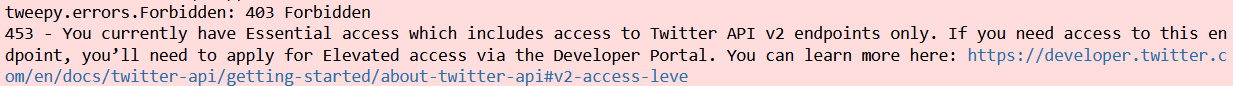
\includegraphics[width=0.8\linewidth]{images/Twitter API Forbidden.png}    

    \caption{The error shown when trying to access a Tweet's text without special privileges.}
    \label{fig:Twitter_API_Forbidden} 
\end{figure}

\begin{lstlisting}[language=python, float, caption={Using the Python {\normalfont tweepy} library to get Tweet features from both the Tweet and the author.}, label=lst:tweepy]
    response = client.get_tweets(IDs[batch_ix : min(batch_ix + 100, n)], 
                                         tweet_fields=
                                             ["created_at", "text", "lang", "author_id", "source"],
                                         user_fields=
                                             ["location", "description", "verified"],
                                         expansions="author_id")

\end{lstlisting}

The other features of Tweets that are acquired in Listing \ref{lst:tweepy} using code from \citet{TweepyTutorial} are the ones specified in the request, i.e., the Tweet-specific ones, like $created\_at$ (the data and time that the Tweet was created at), $text$ (the source text of the Tweet), $lang$ (the language of the Tweet), $author\_id$, $source$ (the device that the Tweet was published on, e.g., a mobile device or personal computer), and the user-specific ones, like $location$, $description$, and $verified$ (the verification status of the user), where both sets of features were combined using the id of the author of the Tweet as their user id. 

As can be seen in the Listing, the number of Tweets that can be included in one request is limited to 100, which is why this call was made multiple times with batches of 100 Tweet IDs in each request until the features for all Tweets were gathered.

\subsection{Transformation}

After further analysis, one problematic aspect of the dataset was found to be the diversity of languages present. It was found that 11,708 Tweets (7.34\%) in the training dataset alone were in a language other than English. While a better BERT model like mBERT could support multiple languages and might achieve even better generalisability if the final project could detect fake news in multiple languages, the simpler, English-only BERT model was chosen, which meant that it could only support Tweets made in the English language. This is further explained in Section \ref{sec:improvements}.

Another problem encountered was one that many datasets suffer from: class imbalance. Oftentimes, there is a class that occurs much more frequently than another, and it is the responsibility of the researcher who makes the ML model not to allow for predicting only the majority class every time, which, if the classes are extremely unbalanced, would achieve deceptive results. As discussed in Section \ref{sec:design_dataset}, there are multiple methods of achieving balance between the classes, but because of time constraints, the easiest method of down-sampling was chosen. Therefore, the majority classes were down-sampled as in \citet{ClassImbalance}. 

Because of the Tweets in the dataset often containing the same link to a news article they are referring to, it was vital not to have Tweets relating to the same article in both the training and testing sets because the model would easily learn to just look at the linked article and make decisions based on that. This was the reason that even the simple Logistic Regression model achieved 97\% accuracy before any fine-tuning, which was too good to be true. Therefore, I extracted the \textit{article\_id} for each Tweet in the dataset, grouped it by the article, shuffled and split the Tweets into training, validation, and testing datasets using \textit{GroupShuffleSplit} as from \citet{GroupSplit}, seen in Listing \ref{lst:groupsplit}. As also noticeable in the Listing, a \textit{random\_state} variable was used to keep the evaluation results of the model consistent and not subject to random variation from how the datasets were split.

\begin{lstlisting}[language=python, float, caption={Using the {\normalfont sci-kit learn GroupShuffleSplit} library to split the dataset into a training and validation set\protect\footnotemark and a testing set.}, label=lst:groupsplit]
gs_1 = GroupShuffleSplit(n_splits=1, train_size=.7, random_state=111019)
train_val_ix, test_ix = next(gs_1.split(X, y, groups=X.article_id))
\end{lstlisting}

\footnotetext{This is later split to get the training and validation sets individually, but the code for it (inspired by \citet{GroupSplitVal}) is skipped to avoid repetition.}


\section{Input Building}
\label{sec:imp_input}

As already mentioned above, the two different models required two different inputs to be able to be trained and predict text. The varied input building for the models is discussed below.

\subsection{Logistic Regression-Specific}

For the Logistic Regression algorithm, input that was already in the form of sentences only needed to be vectorised with a vectoriser from some library, which in previous projects was the TF-IDF vectoriser since it proved to be the most effective. The whole process of encoding the input (both for training and testing) is shown in Listing \ref{lst:tf_idf}, which demonstrates how much shorter the code for it is compared to input building for BERT, explained below.

\begin{lstlisting}[language=python, float, caption={Vectorising input for the Logistic Regression algorithm with TF-IDF.}, label=lst:tf_idf]
# Get features for TF-IDF
tfidf = TfidfVectorizer()
tfidf.fit(train_text)
train_features = tfidf.transform(train_text)
test_features = tfidf.transform(test_text)
\end{lstlisting}

\subsection{BERT-Specific}

The reason for input building being much more difficult for BERT in this specific project was the inclusion of multiple features, many of which had different categories: numerical, categorical, and lexical. One of the most important decisions for this project was how to combine all of the different features into a model that accepts all of them. The original idea was to use different feature-engineering methods for each type of feature: numerical features with standardisation of numbers, categorical features with other types of standardisation, and lexical features with Natural Language Processing techniques. This multi-modal approach would have involved not just different types of feature engineering for every feature type, but also a Multi-Layer Perceptron to combine these features and make decisions based on them, as per \citet{MultiModalBert}.

Because the approach outlined above was too unnecessarily complicated for such a project, a much simpler solution was found in \citet{BERTAllFeatures} by including all of the different features as a combined text paragraph for each Tweet, which was built with a template format as seen in Listing \ref{lst:combo}. An example of the format being filled in with one item's information can be found in Figures \ref{fig:bert_prediction} and \ref{fig:new_tweet}.

\begin{lstlisting}[language=python, float, caption={Combining all features into one paragraph per Tweet that BERT can then analyse.}, label=lst:combo]
sen_w_feats = []
for index, row in data_df.iterrows():
    combined = ""
    
    combined += f"I created this Tweet at {row['created_at']} o'clock " + \
        f"in the {row['lang']} language and in {row['location']} " + \
        f"from {row['source']}. "
        
    verification_status = "verified" if row["verified"] else "not verified"
    combined += f"My name is {row['name']}, username is {row['username']} " + \
        f"and I am {verification_status}. "
    
    combined += f"I would describe myself as {row['description']}. "
    
    combined += f"I wrote: {row['text']} "
    
    # Add the combined text to the list.
    sen_w_feats.append(combined)

\end{lstlisting}

After sentences have been made for every Tweet, they have to be encoded with the usual NLP techniques, which are achieved by using \textit{BertTokenizer} from HuggingFace's \textit{transformers} Python library with the sentence as input. As seen in Listing \ref{lst:BERT_encoder}, the tokeniser uses the same parameters that were discussed in Subsection \ref{subsec:BERTTokeniserParams}, i.e., special tokens and attention masks, but other parameters are specified as well to improve consistency (in the case of \textit{max\_length} and \textit{truncation} and efficiency (in the case of \textit{return\_tensors} being \textit{PyTorch} tensors, which are from another package used in the project).

\begin{lstlisting}[language=python, float, caption={Encoding every sentence for BERT input.}, label=lst:BERT_encoder]
input_ids = []
attention_masks = []
# For every sentence...
for sent in sen_w_feats:
    # `encode_plus` will:
    #   (1) Tokenize the sentence.
    #   (2) Prepend the `[CLS]` token to the start.
    #   (3) Append the `[SEP]` token to the end.
    #   (4) Map tokens to their IDs.
    #   (5) Pad or truncate the sentence to `max_length`
    #   (6) Create attention masks for [PAD] tokens.
    encoded_dict = tokenizer.encode_plus(
                        sent,                      # Sentence to encode.
                        add_special_tokens = True, # Add '[CLS]' and '[SEP]'
                        max_length = max_len,           # Pad & truncate all sentences.
                        truncation = True,
                        padding = 'max_length',
                        return_attention_mask = True,   # Construct attn. masks.
                        return_tensors = 'pt',     # Return pytorch tensors.
                )
    
    # Add the encoded sentence to the list.    
    input_ids.append(encoded_dict['input_ids'])
    
    # And its attention mask (simply differentiates padding from non-padding).
    attention_masks.append(encoded_dict['attention_mask'])

\end{lstlisting}


\section{Logistic Regression Model Training}
\label{sec:imp_lr}

As in building input, training the Logistic Regression algorithm was much simpler compared to its BERT counterpart, as seen in Listing \ref{lst:LR_trainig_eval}, where both training and evaluation is fit into 4 lines of code. The \textit{evaluation\_summary()} function is a simple Python function that includes a description and two metrics from the \textit{sci-kit learn} library: Classification report, which includes F1 score, accuracy, and other metrics, and Confusion matrix, explained in Section \ref{subsec:conf_matrix}.

\begin{lstlisting}[language=python, float, caption={Training and evaluating the Logistic Regression algorithm.}, label=lst:LR_trainig_eval]
# Logistic Regression with TF-IDF
lr_tfidf = LogisticRegression()
lr_model_tfidf = lr_tfidf.fit(train_features, train_labels)
lrtfidf_test = lr_model_tfidf.predict(test_features)
evaluation_summary("LR (TF-IDF) test", test_labels, lrtfidf_test)
\end{lstlisting}

\section{BERT Model Training}
\label{sec:imp_BERT}

The BERT training code was adapted from \citet{BERTAllFeatures}.

\subsection{Optimisation}

The model training inspired by \citet{BERTAllFeatures} uses an optimiser called AdamW, which adapts step sizes based on individual weights during training \citep{AdamW}. This optimiser step is important to call before calling the learning rate scheduler step, which also optimises the training of the model by dynamically changing the learning rate hyperparameter.

\subsection{Memory Issues}

One of the biggest issues when trying to implement BERT's training was how much memory the model was needing to encode all of the approximately 200 thousand Tweet (paragraph) training dataset. Neither running the code locally nor on Google's Colaboratory platform with GPU-acceleration helped. Therefore, the solution was to trade memory for speed of training with a parameter called gradient checkpointing, which achieves a balance of two memory-saving techniques: saving all activations on the forward pass of training and recomputing all of them on the backward pass \citep{BERTGradientCheck}. This method, while making training longer, allowed to fit the model into memory and start training it.

\subsection{GPU Acceleration}

After solving the memory issue, the first significant problem was that training on a normal CPU would take about 8 days per epoch (approximated). With the suggested epoch amount of 4, the total time of training would take more than a month. This was a problem needing to be solved immediately, and the solution to slow training with a CPU was to use GPU-accelerated hardware that is built for fast and numerous calculations.

The first attempt at using the GPU for faster processing was with the help of Google's Colaboratory service, which offers free GPU computation for a limited time and amount every month. By moving the computational units, like PyTorch tensors, to the GPU, where they were used for computation, the training time approximation changed from 32 days to about 20 hours (for all 4 epochs). However, their computation limits are always changing, "having dynamic usage limits that sometimes fluctuate" \citep{ColabFAQ}, which meant that it was difficult to find out certain limits and it was also impossible to keep training running for a continuous 20 hour duration without staying awake for the full 20 hours. Therefore, another solution was required.

The second and final attempt at getting GPU-accelerated hardware was using my own personal laptop. The way to use GPU acceleration on a programmatic level is to install Nvidia's Compute Unified Device Architecture (CUDA) Toolkit and the CUDA for Deep Neural Networks (cuDNN) extension, after which there are not many resources online on how exactly to use it since there are various versions for CUDA, cuDNN, and a limitation on the versions of libraries they can be used for, e.g., Hugging Face and PyTorch. Once Nvidia allowed its users to log in \citep{NvidiaLogIn}, only after some time did I find that PyTorch needs to be installed in the environment with a CUDA version nested inside (while mine was already installed for previous projects without CUDA), which then (after an environment restart) allowed PyTorch to finally see and use the GPU available with the message:

\begin{quote}
    There are 1 GPU(s) available.
    
    We will use the GPU: NVIDIA GeForce RTX 2060
\end{quote}

\subsection{Validation Loss}

During the training of the model, validation loss is calculated and output in order to see how well the model performs on unseen (validation) data as a trade-off to performing too well on seen (training) data. This is to perform over-fitting in the long run.

\section{Website Building}
\label{sec:imp_web}

\subsection{Django}

The URL structure is simple and can be seen in Listing \ref{lst:django_url}, where the \textit{home} view uses the \textit{index.html} template and the \textit{result} view uses the \textit{prediction.html} template, both templates inheriting from the \textit{base.html} template.

\begin{lstlisting}[language=python, float, caption={The entire list of pages accessible on the Django-made website.}, label=lst:django_url]
urlpatterns = [
    path('admin/', admin.site.urls),
    path('', project_views.home, name="home"),
    path('result/', project_views.result, name='result'),
]
\end{lstlisting}

The two view functions mentioned in Listing \ref{lst:django_url}, \textit{home()} and \textit{result()}, are the two functions responsible for the two pages users can visit: the home page and the prediction page, respectively. \textit{home()} just displays the \textit{index.html} template, but \textit{result()} takes as input the model chosen by the user and the text input (either just text or a link to a Tweet), builds the appropriate input for the chosen model, uses the model to predict the veracity of the input, and displays the appropriate template with this prediction. 

Standardisation of the pages the users can visit can be achieved by taking advantage of the aforementioned template inheritance offered by Django, which allows setting a base template that all (or any number of) other templates will use, with specific blocks set in place for customisation. For example, seen in Listing \ref{lst:base_template} is the title HTML tag in \textit{base.html}, which includes a block for customising the specific tab title of each page, like "Home page" for \textit{index.html} and "Prediction" for \textit{prediction.html}. The full template can be found in Appendix \ref{app:base_template}, which includes linking Bootstrap for implementing a more modern UI and another example of inheritance.

\begin{lstlisting}[language=HTML, float, caption={Using Django template inheritance in {\normalfont base.html} to have a standardised interface between the two available templates.}, label=lst:base_template]
<title>
    
    
</title>

\end{lstlisting}

\subsection{User Interface}

The home page can be seen in Figure \ref{fig:home_page}. A lot of white space was used around the core functionality of the fake news detection tool in order for the user not to be overwhelmed with too much functionality and bloat, similarly to Google Search's simplistic approach. Instead, the core elements were kept for the user to interact with: the title of the website, Fake News Classification, which always redirects the user to the home page; the two radio select buttons for the user to choose between which type of model they want to use; the input text area either for the text of the Tweet in the case of Logistic Regression or for the link of the Tweet in the case of BERT; and, finally, the submit button. In every piece of writing on the website, simple language is used for the average, non-technical user to understand, which is why Logistic Regression nor BERT is ever mentioned, but their characteristics (text-only or feature-rich, respectively) are used.

\begin{figure}
    \centering
    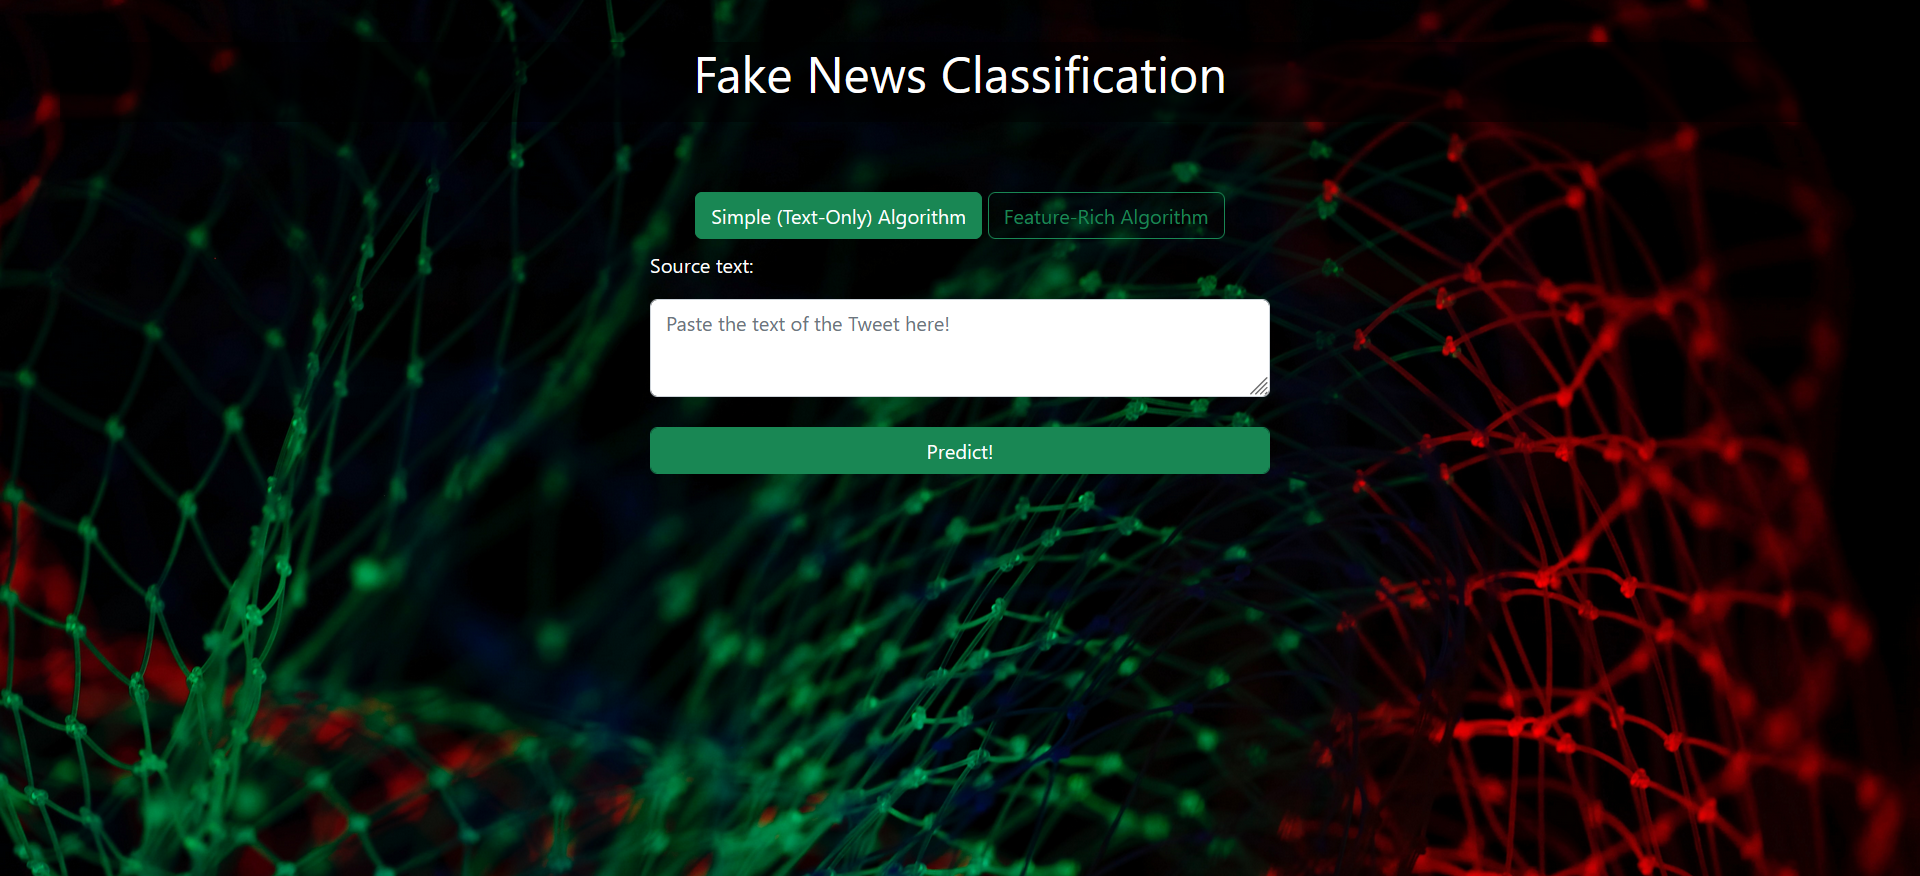
\includegraphics[width=1\linewidth]{images/web/home.png}    

    \caption{The home page of the website with the Logistic Regression model chosen.}
    \label{fig:home_page} 
\end{figure}

The prediction of the input by the Logistic Regression model can be seen in Figure \ref{fig:lr_prediction} for a fake news Tweet taken directly from the dataset. As visible in the Figure, not only is the prediction of the model shown, but the user can also see what exactly was analysed to get that prediction, i.e., they can see the input text they entered at the same time as the prediction. While it is less beneficial to see the same exact text while using the Logistic Regression model, the benefits of this can be better seen in the case of the BERT model, as seen below.

\begin{figure}
    \centering
    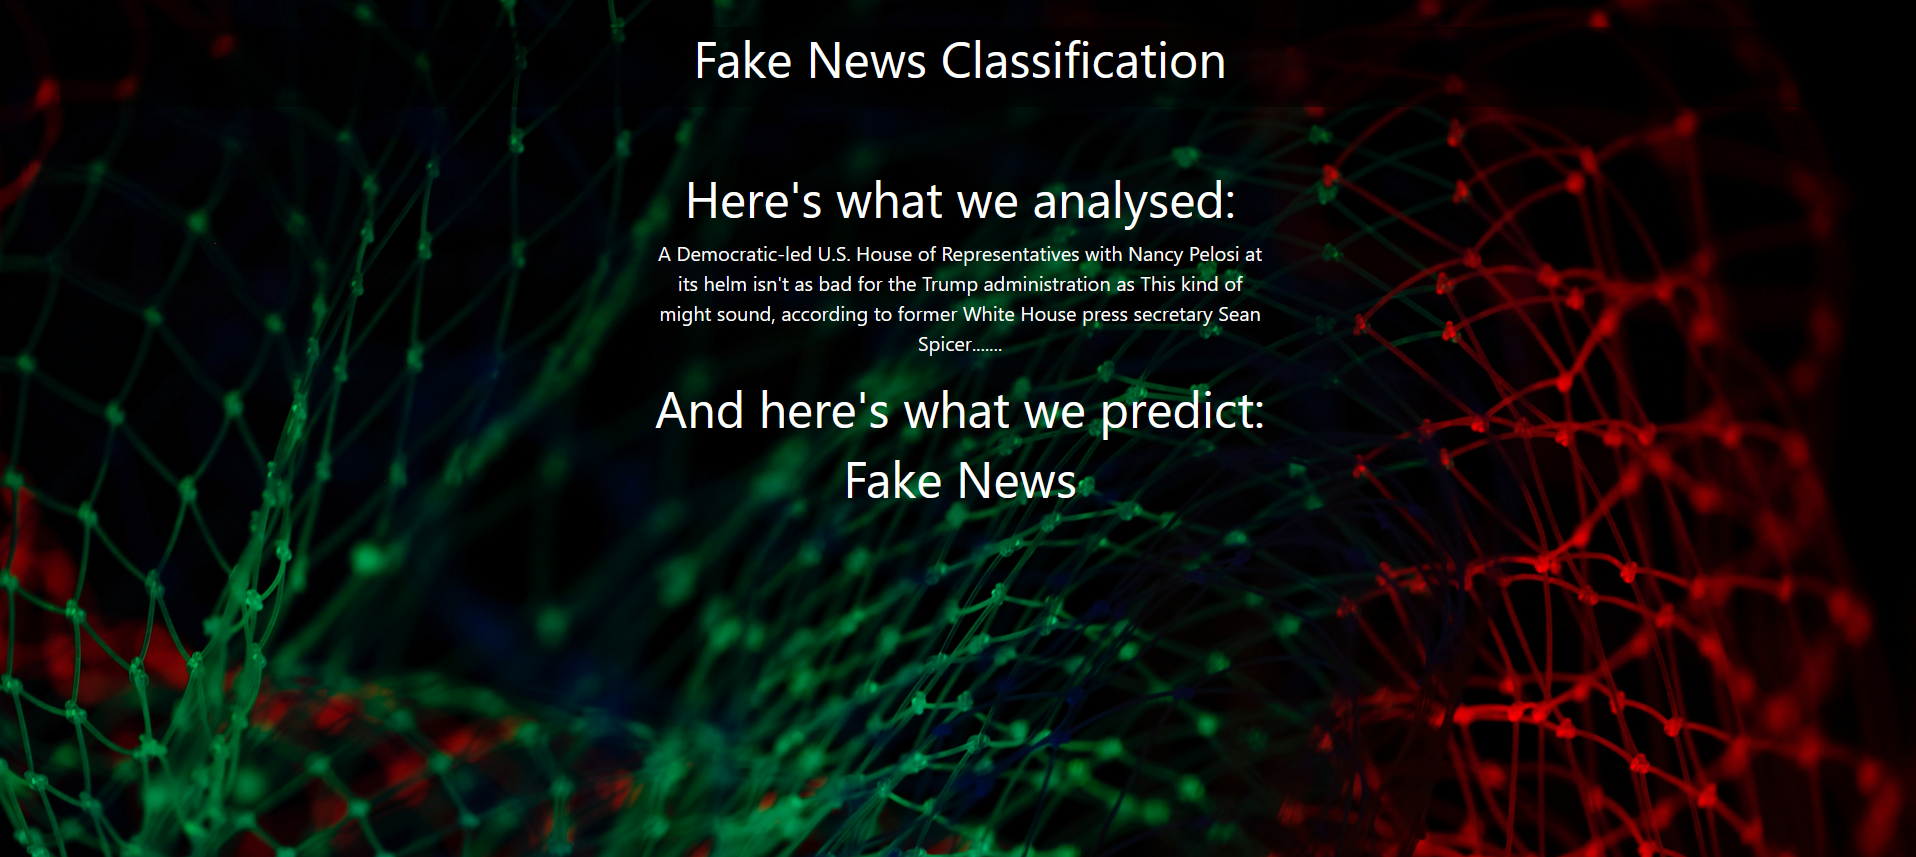
\includegraphics[width=1\linewidth]{images/web/lr.png}    

    \caption{The prediction of text-only input by the LR model.}
    \label{fig:lr_prediction} 
\end{figure}

The prediction of a real news Tweet taken from the dataset by the BERT model can be seen in Figure \ref{fig:bert_prediction}. As visible in the Figure, the resulting paragraph from all features being combined into one text (outlined in Subsection \ref{subsec:dataset_anal}) is displayed to the user, who can see exactly what is analysed to get BERT's prediction of the Tweet they submitted as input.

\begin{figure}
    \centering
    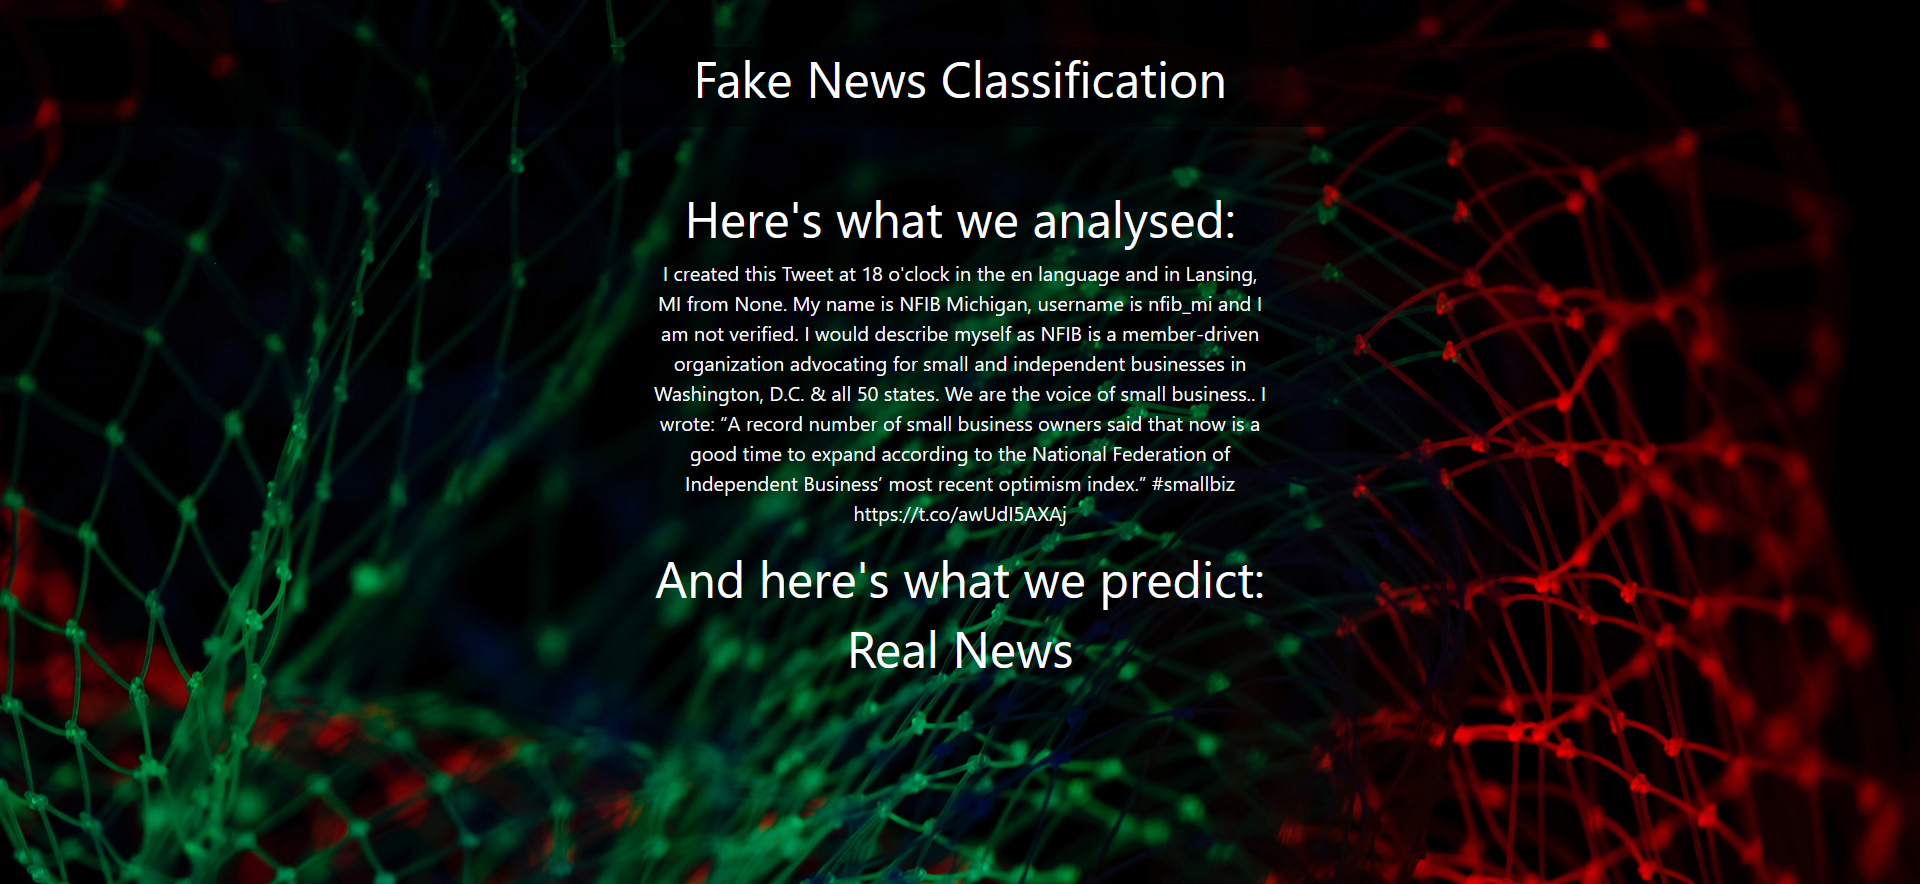
\includegraphics[width=1\linewidth]{images/web/bert.png}    

    \caption{The prediction of the Tweet link input by the BERT model.}
    \label{fig:bert_prediction} 
\end{figure}

To change the placeholder text of the input area for the user according to what type of model they have chosen, jQuery was used in conjunction with setting the \textit{name} attributes of the radio select elements to \textit{model\_select}, while also specifying their respective values in the \textit{value} attribute of the HTML tag. With these elements and attributes in place, tag selection could be used to find and change the text area's placeholder with the code shown in \ref{lst:jquery}.

\begin{lstlisting}[language=JavaScript, float, caption={Changing the input field's placeholder according to which model has been chosen using {\normalfont jQuery}.}, label=lst:jquery]
$('input[type=radio][name=model_select]').change(function() {
    if (this.value == 'simple_model') {
        $('form').find("textarea[type=text]").each(function(){
            $(this).attr("placeholder", "Paste the text of the Tweet here!");
        });
    }
    else if (this.value == 'complex_model') {
        $('form').find("textarea[type=text]").each(function(){
            $(this).attr("placeholder", "Put the link of the Tweet here!");
        });
    }
});

\end{lstlisting}


\subsection{Form Submission}

The input for the BERT model on the website is a simple link to a Tweet that the user wants to analyse. In order to fetch that Tweet's features programmatically, the ID of the Tweet is acquired from the provided link with the help of a regular expression (regex) as seen in Listing \ref{lst:regex}, which, if found, is passed to the aforementioned \textit{tweepy} client that fetches the features of the Tweet for analysis by BERT. As seen in the Listing, the regex finds all numbers after a certain phrase and assumes the correct one is the first because there can be many extra numbers attached to the URL passed in from referral links, etc. Additionally, the regex depends on the URL scheme of Twitter not changing in the near future because, as of March 2023, the ID of the Tweet follows directly after the \textit{/status/} subdirectory. If a user submits an incorrectly formatted link or the URL scheme changes, the prediction returns the error "That does not seem to be a valid link to a Tweet." to the user. If the Tweet is removed from Twitter, as sometimes happens especially to fake news Tweets that become popular, the prediction shows "It seems that the Tweet has been removed." to the user.

\begin{lstlisting}[language=python, float, caption={Using a regular expression to find the ID of the Tweet from a link to it.}, label=lst:regex]
regex_numbers = re.findall('/status/(\d+)', link)
    if len(regex_numbers) == 0:
        return "no link"
    tweet_id = regex_numbers[0]

\end{lstlisting}

\clearpage

%==================================================================================================================================
\chapter{Evaluation}
\label{chap:eval}
% How good is your solution? How well did you solve the general problem, and what evidence do you have to support that?

% Make sure you present your evidence well. Use appropriate visualisations, reporting techniques and statistical analysis, as appropriate.

\section{Evaluation Metrics}

\subsection{Standard Performance Metrics}

Evaluation of the previously implemented models should take into account the performance of the baseline model. While training the two models, an additional "DummyClassifier" from the \textit{sci-kit learn} library was trained, which counts only the frequency of tokens and nothing else. As can be seen in Figure \ref{fig:DummyModel} and as expected, its accuracy is little more than 50\%, which is almost as good as guessing 50-50, and its F1 score is a low 35.6\%. As can also be seen in the Figure, the baseline model could only predict all Tweets as Real News.

\begin{figure}
    \centering
    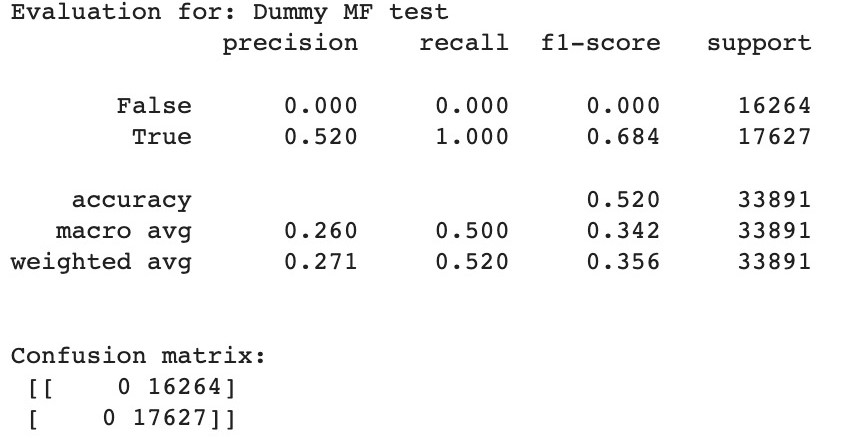
\includegraphics[width=0.8\linewidth]{images/Evaluation/DummyMostFrequentCrop.jpg}    

    \caption{Standard performance metrics and confusion matrix for the Dummy Most-Frequent (MF) baseline model.}
    \label{fig:DummyModel} 
\end{figure}

The final accuracy of the Logistic Regression algorithm was \textbf{82.8\%}, with the F1 score being \textbf{82.6\%}. As expected, the performance of such a simple model with only one feature being analysed is moderately better than the performance from the earlier \textit{PHEME} dataset, which had an F1 score of 61.2\%. As for the BERT model, its F1 score and accuracy were much higher: \textbf{99.4\%} and \textbf{99.2\%}, respectively. This dramatic increase in performance is partly due to the incredible pre-training of BERT with 80 million tokens and its state-of-the-art architecture of a transformer model, but also because of multiple features being used instead of just the text of a Tweet. The drawback of such a high performance score, compared to the scores achieved in literature with models having been trained with more resources and bigger datasets, is that it is almost definitely too high to be viably generalisable to new input. This is discussed further on.

\subsection{Confusion Matrix}
\label{sec:ConfMatrix}

\begin{figure}
    \centering
    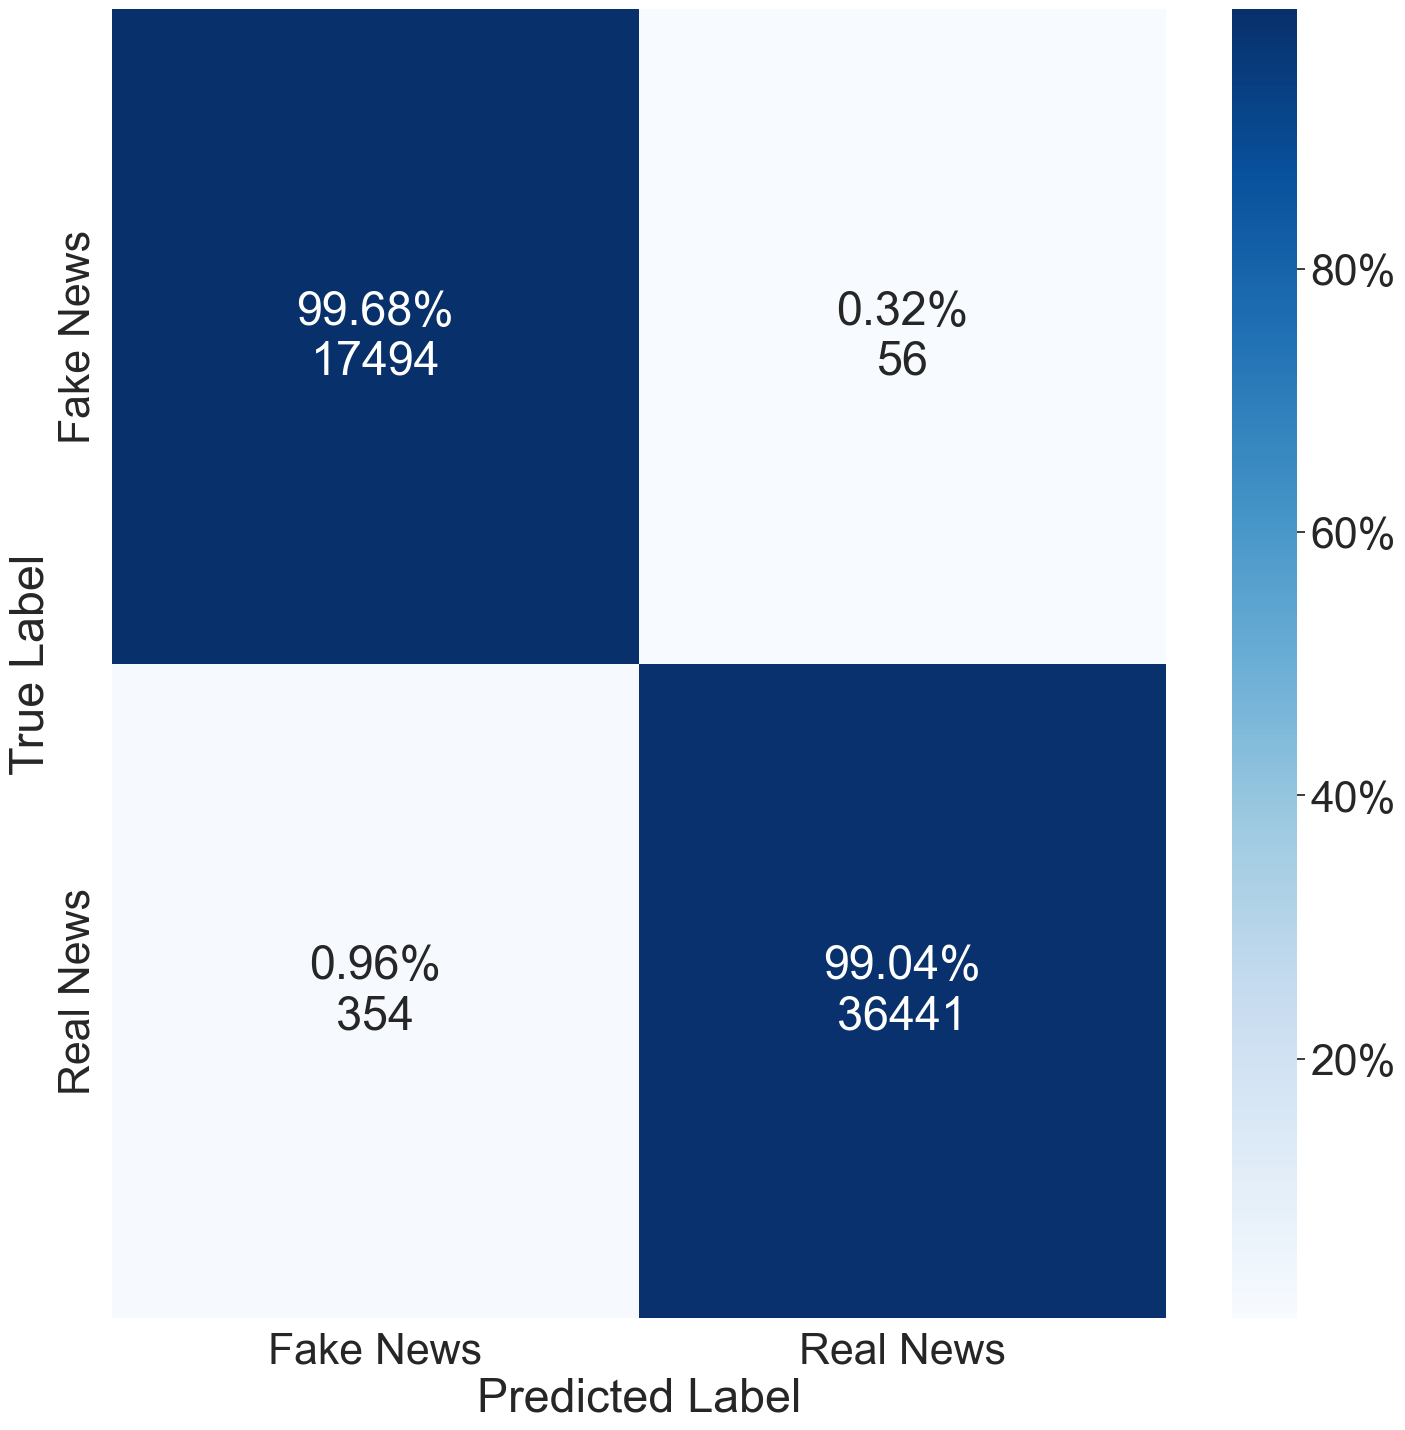
\includegraphics[width=0.8\linewidth]{images/Evaluation/conf_matrix_w_pct.png}    

    \caption{A standardised confusion matrix for BERT after final training.}
    \label{fig:eval_confusion_matrix} 
\end{figure}

\begin{figure}
    \centering
    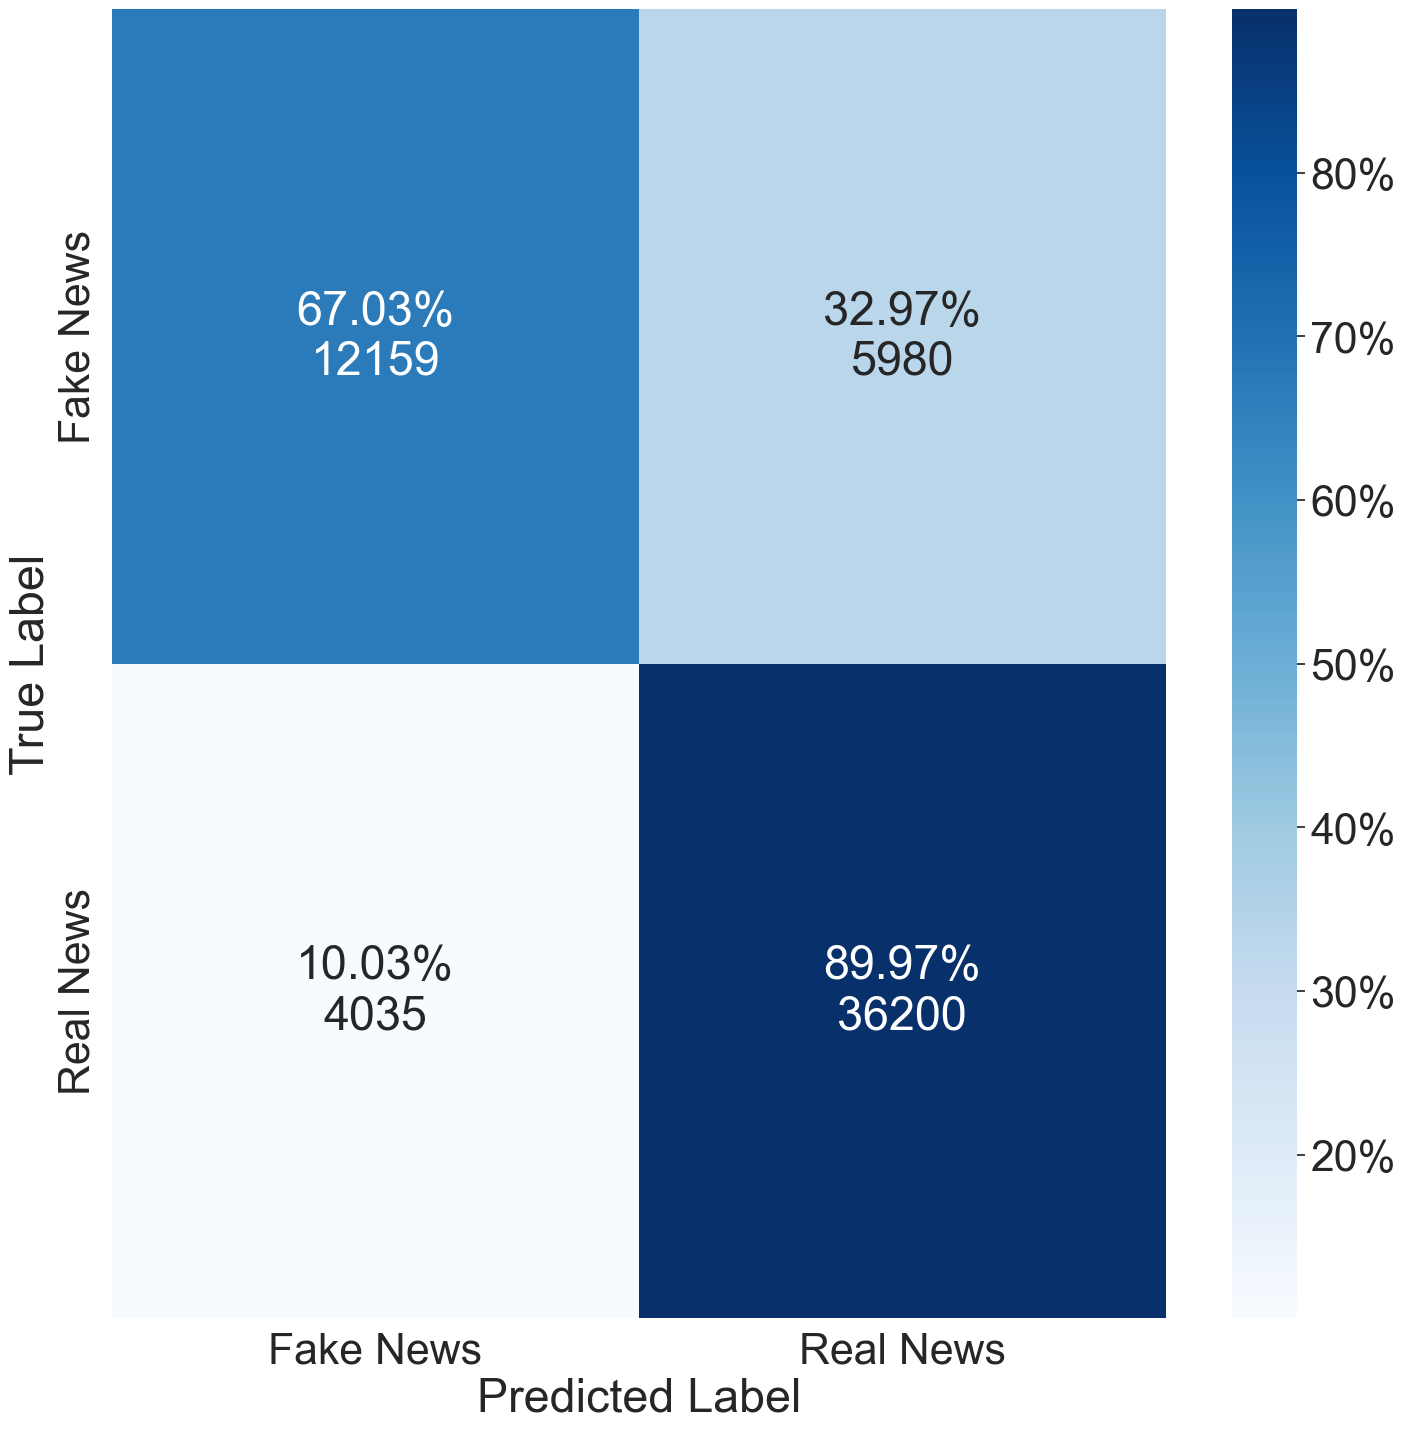
\includegraphics[width=0.8\linewidth]{images/Evaluation/LR conf matrix.png}    

    \caption{A standardised confusion matrix for the Logistic Regression model.}
    \label{fig:eval_LR_confusion_matrix} 
\end{figure}

The confusion matrix for the Logistic Regression model is shown in Figure \ref{fig:eval_LR_confusion_matrix}. As can be seen, the confusion matrix reflects LR's accuracy and F1 score, but is also predicting more fake news as real news than vice versa, the skewing of which, while ideally not being skewed either way, is problematic for users who will believe the prediction of the model.

The confusion matrix for the BERT model is demonstrated in Figure \ref{fig:eval_confusion_matrix}, the code for creating it being adapted from \citet{ConfMatrixPct}. As seen in the Figure, at least 99\% of both classes (Fake and Real) are predicted correctly, while less than 1\% are not. This is reflected in the accuracy and F1 score of the model. As can also be seen by comparing the counts for both classes, the amount of fake news Tweets in the testing dataset is less than half of real news Tweets, which, while it may seem to cause a class imbalance, is not used in the further training of the model, meaning that there is no impact on the model by an imbalanced testing dataset.

When comparing the percentage errors for false predictions, it can be seen that there are about 3 times more real news being predicted as fake news, which signifies that the matrix is skewed towards predicting a Tweet as fake news. While, ideally, this skew should be fixed, there were no solutions found, and, as per the \textit{Could Have} non-functional requirement in Section \ref{sec:non-func_reqs}, this was left as is. Furthermore, real news being mislabelled as fake news can also be seen as a benefit to the user as they are encouraged to scrutinise news that they read (especially on Twitter), while labelling fake news as real news might lead them to trust the fake news even more than before using the tool.


\section{Generalisability}

If I had to choose the most important evaluation metric for a Machine Learning model's performance, it would be its ability to be generalisable to new input that it has not seen before. The more generalisable a model is, the better the likelihood that users would find the tool useful and want to improve their lives with it. While the confusion matrix is useful for testing the model's performance on a testing set that is similar to the training dataset, the training and validation losses over time and the model's performance on a new set of testing values give valuable insight into how useful the tool will be to users.

\subsection{Losses During Training}

The training and validation losses during the training of the model are demonstrated in Figure \ref{fig:eval_losses}. As can be seen in the 4 epochs that were implemented, the training loss continued decreasing until the very last epoch, where it did not noticeably change. In the very last epoch, however, it is visible that the validation loss increased to a value equal to the first epoch's value. This increase in the validation loss signifies that the amount of epochs chosen was too high, resulting in the model being over-fitted to the training dataset. As explained in Section \ref{sec:epoch_amount_param}, over-fitting means that the dataset is too dependent on the training dataset and is therefore less generalisable to new, never before seen input. 

\begin{figure}
    \centering
    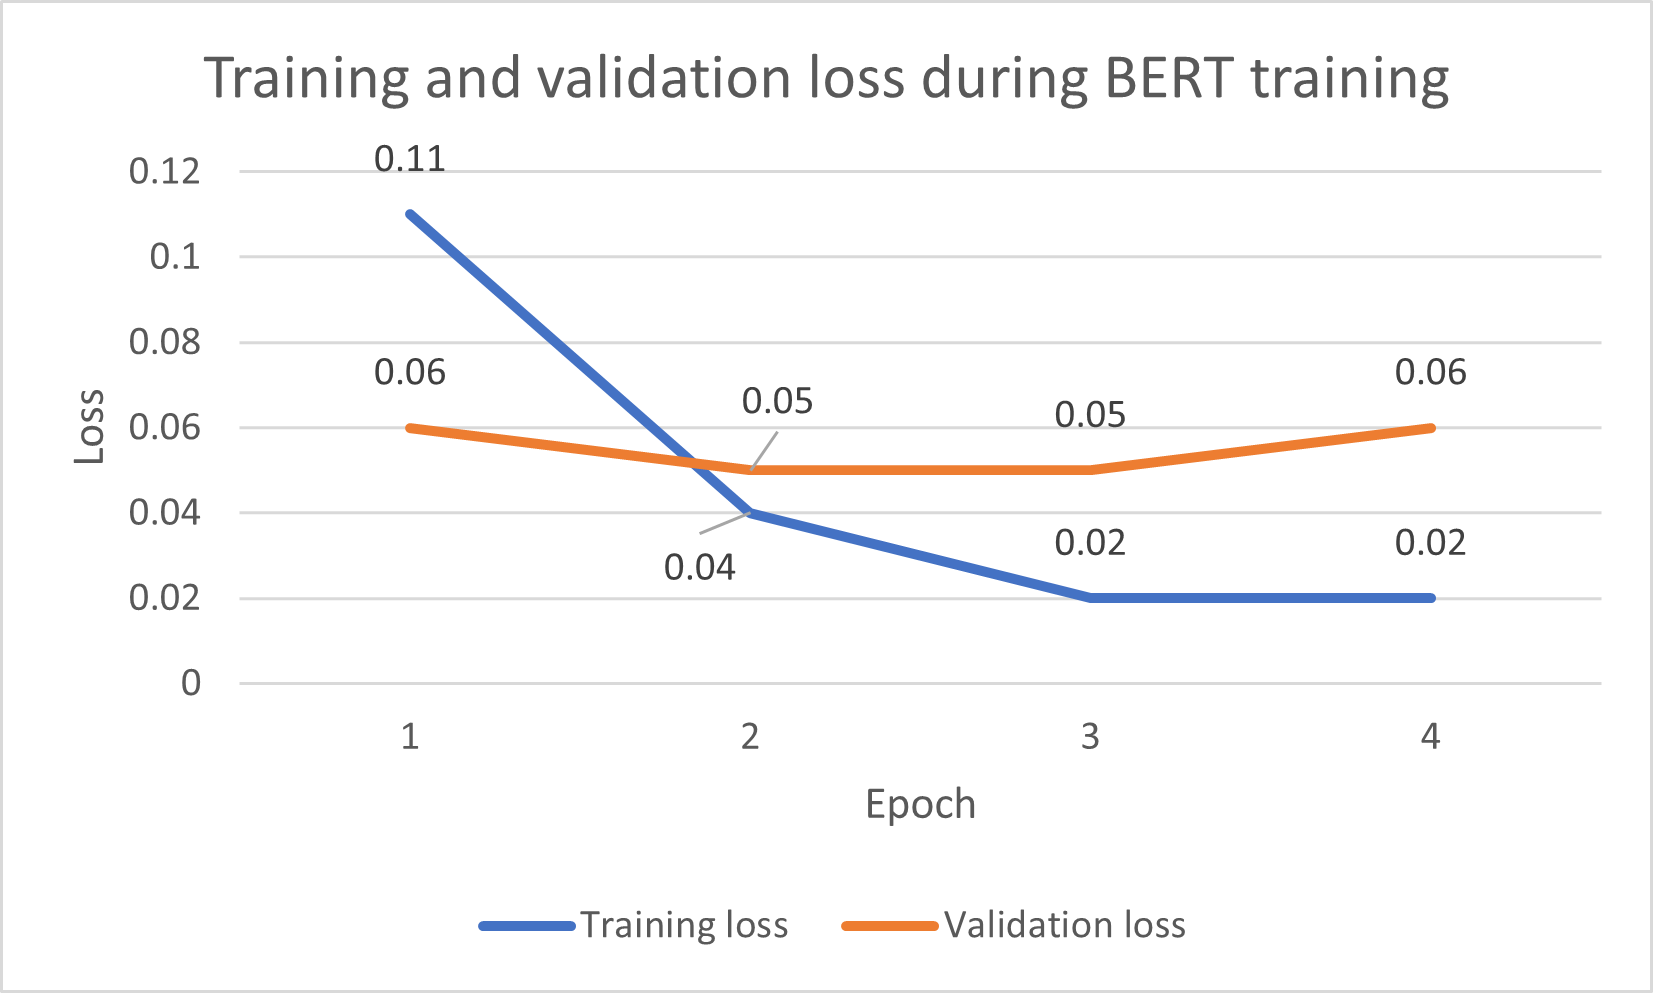
\includegraphics[width=0.8\linewidth]{images/Evaluation/trainingLosses.png}    

    \caption{The losses during BERT training in each epoch.}
    \label{fig:eval_losses} 
\end{figure}

\subsection{Modern Input}
\label{subsec:modern_input}

To check how the models perform with unseen and modern Tweets, a Tweet from a PolitiFact article by \citet{PFBillGates} was chosen, which was labelled as \textit{False} by PolitiFact's Truth-O-Meter score. The BERT model's correct prediction can be seen in Figure \ref{fig:new_tweet}, while Logistic Regression model's prediction was also correct. However, for many other modern fake news Tweets (ones which were not removed because of their infamy, which has happened to many of them due to them being featured on PolitiFact or becoming viral online in general), the prediction was incorrectly attributed as real news. This could be explained by the Tweet in the Figure containing the person-phrase "Bill Gates", which appears more than 50 times more in fake news Tweets than real news ones. This and more phrases are analysed in Appendix \ref{app:phrase_anal}. As can be seen, in many cases, politically significant phrases are featured in one class more often than the other, which means that the model has been trained to associate those phrases with the class they are more frequent in.

\subsection{Potential Reasons Why}

Since evaluations leads us to believe that the model is over-fitted to the data, an investigation should be done into the reasons why this is so and how it could be remedied. The three possible reasons why the model is over-fitted are thus: the Twitter character limit change, different political topics, and different phrases for each class.

Firstly, the FakeNewsNet dataset was collected in 2018, one year after the Twitter character limit was increased from 140 to 280 characters. This, however, is another recent policy change with Twitter again increasing the character limit to 4,000 characters for a select user subset \citep{TwitterCharLimit}. These two increases change not only the literal formatting of the Tweet, but also the way that the authors write the Tweet in its language, particularly, conciseness.

Secondly, the political landscape has changed since 2018, with different topics being discussed now and a change in the prominence of even the same topics. Since only political Tweets were used in the dataset, modern Tweets would obviously have very different topics than in 2018.

Finally, even the phrases in the existing dataset help the model lean towards real news or fake news for a particular Tweet containing these phrases. As discussed in Section \ref{subsec:modern_input}, more analysis than just the one in Appendix \ref{app:phrase_anal} should be done, which afterwards should be used for a more standardised dataset that focuses on language alone.

\begin{figure}
    \centering
    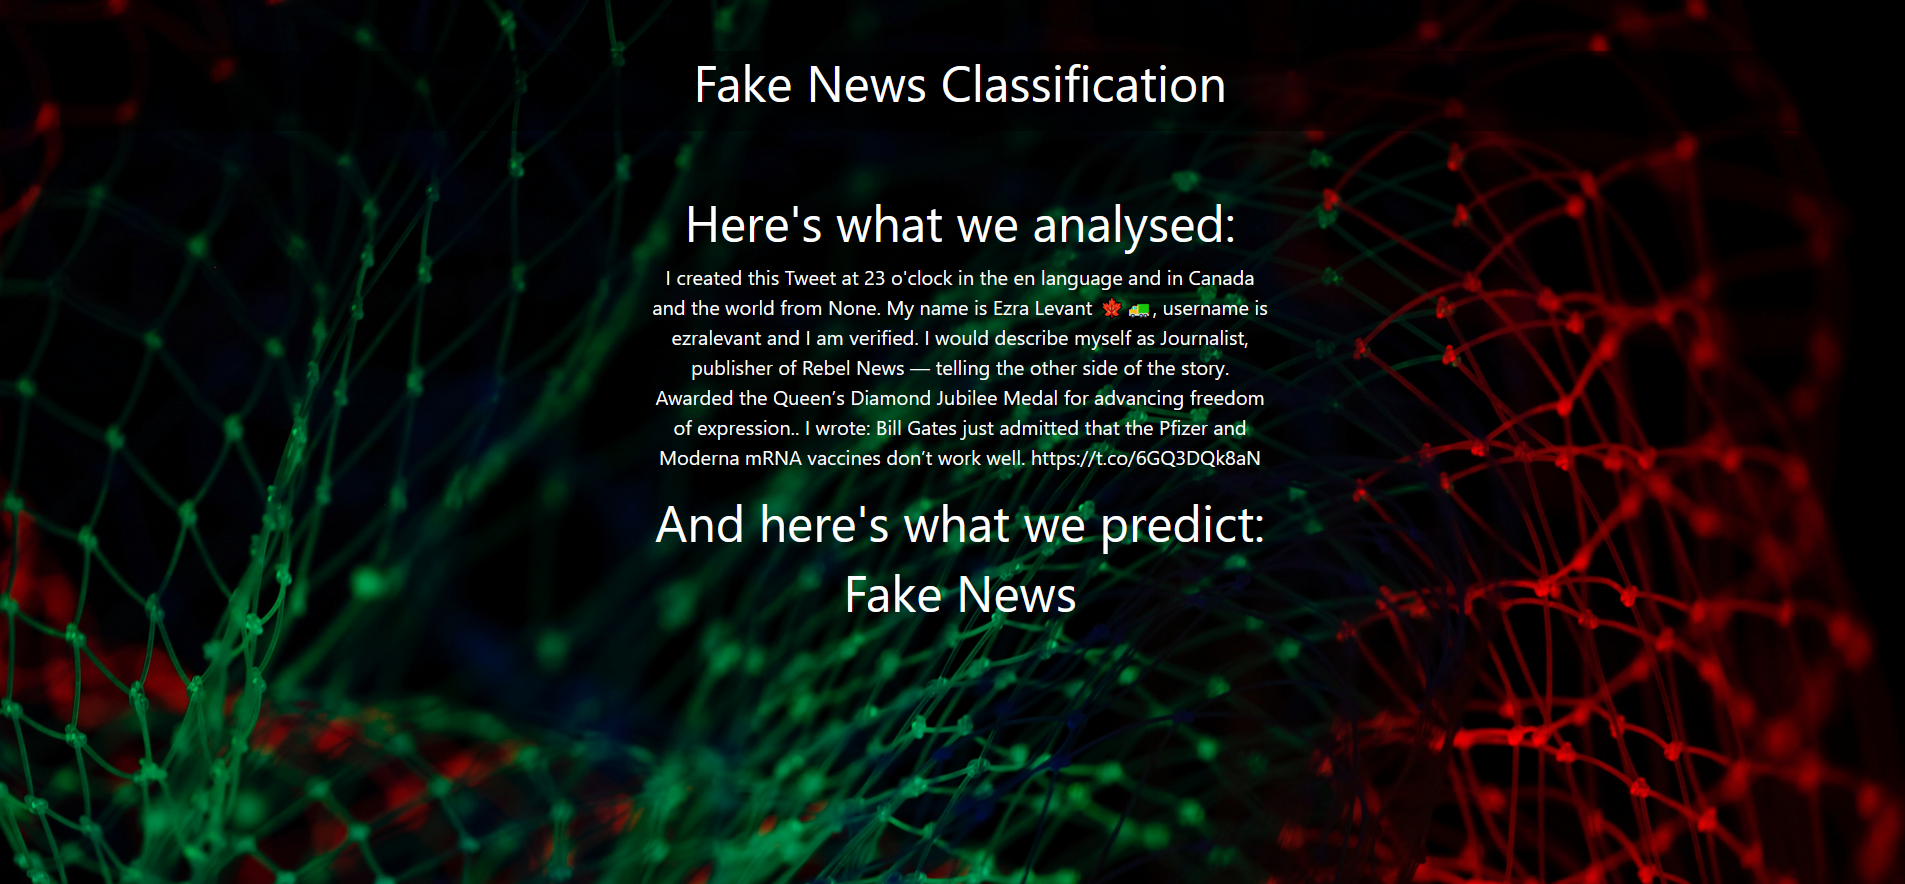
\includegraphics[width=1\linewidth]{images/web/new.png}    

    \caption{BERT model's prediction on the veracity of the Bill Gates vaccine Tweet.}
    \label{fig:new_tweet} 
\end{figure}

\section{Further Improvements}
\label{sec:improvements}

As mentioned previously, since the dataset came with about 7.34\% of Tweets present being in foreign languages, a significant portion of valuable information was lost only because a standard BERT model was chosen and integrated into the project. In order to include these Tweets, it would be beneficial to choose a multilingual model like mBERT for similar datasets not to lose important information. At the minimum, it would also be possible to incorporate a BERT model that supports the second-most frequent language found in the dataset, Japanese, as in \citet{BERTJapanese}.

Another improvement, stemming from analysing the confusion matrix, would be to fix the skewed nature of incorrect predictions to permit about an equal amount of false positives as false negatives. This could be done by analysing certain phrases that might be skewing the model predictions, like in Appendix \ref{app:phrase_anal}.

Additionally, as seen during evaluation, the validation loss of BERT increased in the final epoch, which means it suffered from over-fitting. During the next training of the model, the losses should be kept in a data structure and the training loop should stop in case the validation loss stays the same or even increases in an epoch, which would reduce the overall over-fitting.

The final improvement worth mentioning is the missed \textit{Will not Have} functional requirement of continuously improving and fine-tuning the model with user input about how well the model predicted the Tweet. This improvement, while being difficult to implement with the delicate nature of user trust and avoidance of misuse, would be an invaluable asset to the project as it would greatly reduce over-fitting because of Tweets being widely varied and it would allow the models to learn continuously as the fake news landscape on Twitter and other social media platforms changes.


%==================================================================================================================================
\chapter{Conclusion}  
\label{chap:conclusion}
% Summarise the whole project for a lazy reader who didn't read the rest (e.g. a prize-awarding committee).

The Internet has seen an exponentially increasing rise of fake news propagation on every social media platform there is, especially on Twitter now that it is both a frequent source of news for its users and a company with changing leadership, leading to fluctuating policies on fake news detection and reduction.

In order to help Twitter users distinguish between fake and real news, who are about 54\% accurate at doing so in general, we proposed to build a usable tool to detect fake news in Tweets, with a Machine Learning model that uses Natural Language Processing as the driving decision-maker. The models were then evaluated with standard Machine Learning evaluation metrics, like accuracy, F1 score, and confusion matrix, and then built into the website, which was hosted online. 

To do this, a dataset with about 400,000 Tweets was acquired, analysed, and transformed to extract multiple features of a Tweet, like its text, source, language, and its author's description and verification status. These features were then processed and encoded as input for two different models: Logistic Regression and BERT, a modern Natural Language Processing model with a transformer architecture. 

The models were then trained with the given input. Multiple techniques were used to optimise their performance, like TF-IDF vectorising for the Logistic Regression model and AdamW optimising for the BERT model. Additionally, validation loss was used to reduce over-fitting.

Afterwards, the models were evaluated on their performance. While Logistic Regression achieved only \textbf{82.8\%} accuracy and an F1 score of \textbf{82.6\%}, BERT's accuracy was \textbf{99.2\%}, with an F1 score of \textbf{99.4\%}. While this seems like an impressive score for the dataset, this high of an F1 score implies over-fitting of the model to the given dataset, which is demonstrably shown by not correctly predicting modern fake news Tweets acquired from PolitiFact.

These models were then saved and put into a Django website with Bootstrap, a modern CSS framework, and then hosted on a website. It is available here: \url{http://fakenewsuofg.pythonanywhere.com}.

With all \textit{Must Have} and \textit{Should Have} requirements in place, this project provides a contribution to the fields of Machine Learning, Natural Language Processing, and, more specifically, Fake News Detection by creating and spreading awareness of an online tool for people to use to help them detect fake news online by simply copy-pasting the text or link of a Tweet into the tool and letting the model analyse it for them. This can then act as a stepping-stone for stronger integrity of news online.

%==================================================================================================================================
%
% 
%==================================================================================================================================
%  APPENDICES  

\begin{appendices}

\chapter{Twitter API Educational Access Form}
\label{app:Twitter_Education}

\textbf{How will you use the Twitter API or Twitter Data?}

My dissertation project in my final year as an undergraduate University of Glasgow student is about using Natural Language Processing in Machine Learning to build a model that could tell fake and real news distributed on social media apart. As Twitter is a very widely used platform to spread misinformation by malicious users, I want to extract features from Tweets that could be useful in building such a model, like the source text and the time they were posted. With this model, I plan to create a tool (so far the plan is for a website) for users to input the text or URL of a Tweet to better understand whether that Tweet is likely to be fake news, which would hopefully reduce the spread of misinformation on social media.

GitHub link: https://github.com/xid-er/Fake-News-Detection

\textbf{Please describe how you will analyze Twitter data including any analysis of Tweets or Twitter users.}

I plan to extract specific features from Tweets in the fake and real news-annotated dataset I have to build a machine learning model with BERT preprocessing and a Linear Regression model. The features will be: source text, creation time, user description and verification status.

\textbf{Please describe how and where Tweets and/or data about Twitter content will be displayed outside of Twitter.}

The information about these Tweets will be aggregated into the dataset analysis section of my dissertation, which may or may not be published in the end. The same data mentioned above will be analysed, but any usernames or other types of sensitive information will be removed from publication.


\chapter{Base Django Template for Website}
\label{app:base_template}

Displayed in Listing \ref{lst:base_template_full}.

\begin{lstlisting}[language=HTML, float, caption={The base template, using inheritance in the title and body blocks, with Bootstrap linked in the template.}, label=lst:base_template_full]
<!DOCTYPE html>


<html lang="en" dir="ltr">
  <head>
    <meta charset="utf-8">

    <title>
        
        
    </title>
    <link rel="stylesheet" href="" />
    <link rel="shortcut icon" type="image/png" href=""/>
    <link href="https://cdn.jsdelivr.net/npm/bootstrap@5.2.3/dist/css/bootstrap.min.css" rel="stylesheet" integrity="sha384-rbsA2VBKQhggwzxH7pPCaAqO46MgnOM80zW1RWuH61DGLwZJEdK2Kadq2F9CUG65" crossorigin="anonymous">
  </head>
  <body id="header" style="--bs-bg-opacity: .8;">
    <header>
      <div class="p-5 text-center">
        <div class="mask" style="background-color: rgba(0, 0, 0, 0.5);">
          <div class="d-flex justify-content-center align-items-center h-100">
            <div class="text-white">
              <h1 class="mb-3"><a class="text-white text-decoration-none" href="">Fake News Classification</a></h1>
            </div>
          </div>
        </div>
      </div>
    </header>
    
    
    <script src="https://cdn.jsdelivr.net/npm/bootstrap@5.2.3/dist/js/bootstrap.bundle.min.js" integrity="sha384-kenU1KFdBIe4zVF0s0G1M5b4hcpxyD9F7jL+jjXkk+Q2h455rYXK/7HAuoJl+0I4" crossorigin="anonymous"></script>
    <script src="" crossorigin="anonymous"></script>
    <script src="" crossorigin="anonymous"></script>
  </body>
</html>

\end{lstlisting}

\chapter{Dataset Phrase Analysis}
\label{app:phrase_anal}

Bill Gates:
\begin{itemize}
    \item Fake: 608 / 108\_930 (0.56\%)
    \item Real: 44 / 296\_170 (0.01\%)
\end{itemize}

Trump:
\begin{itemize}
\item Fake: 23\_161 (21.26\%)
\item Real: 59\_694 (20.16\%)
\end{itemize}

Clinton:
\begin{itemize}
\item Fake: 3049 (2.80\%)
\item Real: 8842 (2.99\%)
\end{itemize}

Pelosi:
\begin{itemize}
\item Fake: 1295 (1.19\%)
\item Real: 1740 (0.59\%)
\end{itemize}

Vaccine:
\begin{itemize}
\item Fake: 6040 (5.54\%)
\item Real: 568 (1.92\%)
\end{itemize}

\end{appendices}

%==================================================================================================================================
%   BIBLIOGRAPHY   

% The bibliography style is agsm (Harvard)
% The bibliography always appears last, after the appendices.

\bibliographystyle{agsm}

% Force the bibliography not to be numbered
\renewcommand{\thechapter}{0} 
\bibliography{l4proj}

\end{document}
